\begin{savequote}[8cm]
Phantasie ist wichtiger als Wissen, denn Wissen ist begrenzt."

  \qauthor{--- Albert Einstein}
\end{savequote}

\chapter{Cross Section Systematics in \texorpdfstring{\acrshort{dune}}{TEXT}}

\begin{center}
\textbf{Abstract\\}
\end{center} \vspace{-4mm}
For the operation of precision neutrino experiments, the understanding of neutrino interactions with matter %as well as related cross sections
are preconditioned requirements of all detections and measurements of neutrinos. The largest uncertainties in estimating neutrino-nucleus interaction cross sections arise in the incomplete understanding of nuclear effects. %In order to theoretically predict and experimentally understand data associated with neutrino-nucleus cross sections, the \acrshort{genie} neutrino event generator performs simulations of neutrino interactions according to underlying theoretical models. 
In the study of neutrino oscillations and nuclear scattering processes, obtaining an interaction model with associated uncertainties is of substantial interest for the neutrino physics community. %A comparison of chosen variable distributions from a GENIE simulation with experimental data may allow to discriminate between different nuclear models and to decide which theoretical model to use for data analyses in DUNE.
This report presents studies of simulated \acrshort{cc} \acrshort{2p2h} interactions, in which a neutrino interacts with a bound pair of nucleons. This interaction mode is very poorly constrained by current data. A comparison of three leading \acrshort{cc} \acrshort{2p2h} models is presented, along with a number of uncertainty parameters that have been implemented to account for model-to-model discrepancies in the DUNE oscillation analysis.

% Brief general introduction specifying the purpose of your work
\vspace{-2mm}
\section{Introduction} \label{introduction_syst} \vspace{-3mm}
An essential requirement for high precision measurements in current and future neutrino experiments is the understanding of neutrino-matter interactions. A variety of theoretically-challenging scattering processes and nuclear effects complicate the precise calculation of neutrino-nucleus interaction cross-sections. The leading source of systematic uncertainties are deficiencies in existing models that aim to predict these processes and effects \cite{Alvarez_Ruso_2018,Benhar:2013bwa,Megias:2019pol,PhysRevD.92.051302,Lu:2018stk,Munteanu:2019llq}.
Obtaining a better understanding of this physics at accelerator neutrino energies is a main goal of current experimental collaborations~\cite{Dolan:2018zye,Formaggio:2013kya,PhysRevC.94.015503,Furmanski:2016wqo,Katori:2016yel}. The motivation of the project presented in this report is to carry out neutrino oscillation studies in the \acrfull{dune}, a next-generation long-baseline neutrino experiment.
In the Standard Model of Particle Physics the three generations (flavors) of neutrinos correspondent to three weak eigenstates $\ket{\nu_\alpha}$ of flavor $\alpha = \{\text{e},\mu,\tau\}$. The basis of these weak eigenstates can be related to the basis of mass eigenstates $\ket{\nu_i}$ with $i=\{1,2,3\}$, each with mass $m_i$, by the unitary \acrshort{pmns} matrix $U_{\alpha i}$ \cite{Kayser:2005cd}:
\vspace{-4mm}%
\begin{align} \label{pmns_syst}
\ket{\nu_\alpha} =  U^\dagger_{\alpha i}\ket{\nu_i} \quad \Leftrightarrow \quad \ket{\nu_i} =  U_{\alpha i}\ket{\nu_\alpha} \quad 
\text{with} \quad U_{\alpha i} =
\begin{pmatrix}
    U_{\text{e}1} & U_{\text{e}2} & U_{\text{e}3} \\
    U_{\mu 1} & U_{\mu 2} & U_{\mu 3} \\
    U_{\tau 1} & U_{\tau 2} & U_{\tau 3}
\end{pmatrix}
\end{align}
%
%The flavor-$\alpha$ fractions of the mass eigenstates are shown in \cref{fig:mass_hierarchy}.
The neutrino oscillation parameters are extracted via the neutrino oscillation probability. The probability for a neutrino of mass eigenstate $\nu_i$ to produce a charged lepton of flavor $\alpha$ resulting from a \acrfull{cc} interaction in a detector is given by $|U_{\alpha i}|^2$. The neutrino event rates for $\nu_\alpha \rightarrow \nu_\beta$ oscialltions are computed as \cite{doi:10.1146/annurev-nucl-101917-020930}
%
%\begin{small}
\vspace{-3mm}
    \begin{align} \label{nu_osc_prob_syst}
        R_{\alpha\rightarrow\beta}(p_\text{reco}) = \int\displaylimits_{E_\text{min}}^{E_\text{max}} \Phi_\alpha(E_\text{true}) \cdot \sum_{i} \sigma^i_\beta(E_\text{true}, p_\text{reco}) \cdot \sum_{j} N_j \cdot \varepsilon_\beta(E_\text{true}, p_\text{reco}) \cdot P_{\alpha\rightarrow\beta}(E_\text{true}) \ ,
%       N_\text{det} = \Phi(E_\text{true}) \sigma(E_\text{true})    \varepsilon(E_\text{true},E_\text{rec}) P_\text{osc}
    \end{align}
%\end{small}
%\vspace{-2mm}%
where the event rate is a function of the reconstructed kinematic variables $p_\text{reco} \equiv (E_\text{reco}, \mathbf{p}_\text{reco})$, $\Phi_\alpha$ is the neutrino flux of flavor $\alpha$, $\sigma^i_\beta$ is the cross section for a neutrino $\nu_\beta$ of flavor $\beta$ with the target nucleus for interaction $i$, $N_j$ is the number of target nuclei in the detector fiducial volume of type $j$, $\varepsilon_\beta$ is the detector efficiency for flavor $\beta$ and $P_{\alpha\rightarrow\beta}$ is the neutrino oscillation probability for a neutrino to change from flavor $\alpha$ to flavor $\beta$. In order to extract the neutrino oscillation probability via \cref{nu_osc_prob_syst}, oscillation experiments measure %the neutrino flux in their near, pre-oscillation detectors and determine 
event rates and use them to 
constrain the product of neutrino flux, cross section and detector effects. The number of target nuclei as well as the detector efficiencies are determined in their far, post-oscillation detectors. As seen \cref{nu_osc_prob_syst}, the oscillation probability is a function of true neutrino energy $E_\text{true}$ \cite{ALVAREZRUSO20181}. However, the true value has to be inferred from the reconstructed final-state particles. The kinematics of these final state particles are determined from the cross-section of the neutrino-nucleon interaction. Consequently, any bias from the mis-modelling of the neutrino interaction will be directly mapped into a bias of the oscillation parameters.
%Hence, in order to infer the neutrino oscillation probability via \cref{nu_osc_prob_syst}, it is therefore necessary to know the neutrino energy. While the oscillation probability depends on the true neutrino energy $E_\text{true}$ \cite{ALVAREZRUSO20181}, it cannot be known, such that the neutrino energy has to be reconstructed from the kinematic information of \acrshort{cc} neutrino interactions such as the final state of a neutrino-nucleus interaction. %Such a reconstructed neutrino energy $E_\text{reco}$ 
%To calculate the true neutrino energy, we must account for effects %such as the escape of neutral particles, unobserved energy deposition and assumptions of these effects
%that are based on the cross-section model, such that the reconstruction of the neutrino energy implicitly relies on the estimation of the cross section.
%Any uncertainty in the cross-section estimation leads to an uncertainty in the reconstruction of the neutrino energy, which in turn results in an uncertainty in the neutrino oscillation parameters. 
Therefore, the understanding of neutrino-nucleus cross sections is essential in neutrino-oscillation experiments.
%
\begin{figure}[t!]
	\centering
%	\begin{subfigure}[b]{\textwidth}
%	\includegraphics[width=\textwidth]{figures/xsec_Ev_log_legend.pdf}
%	    \includegraphics[width=\textwidth]{figures/xsec_Ev_numu_log_legend.pdf}
%	    \vspace{-6.mm}
%	    \caption{}
%	    \label{inclusive_xsec}
%	\end{subfigure}
%	    \vskip\baselineskip \vspace{-5.mm}
%	\begin{subfigure}[b]{\textwidth}
	    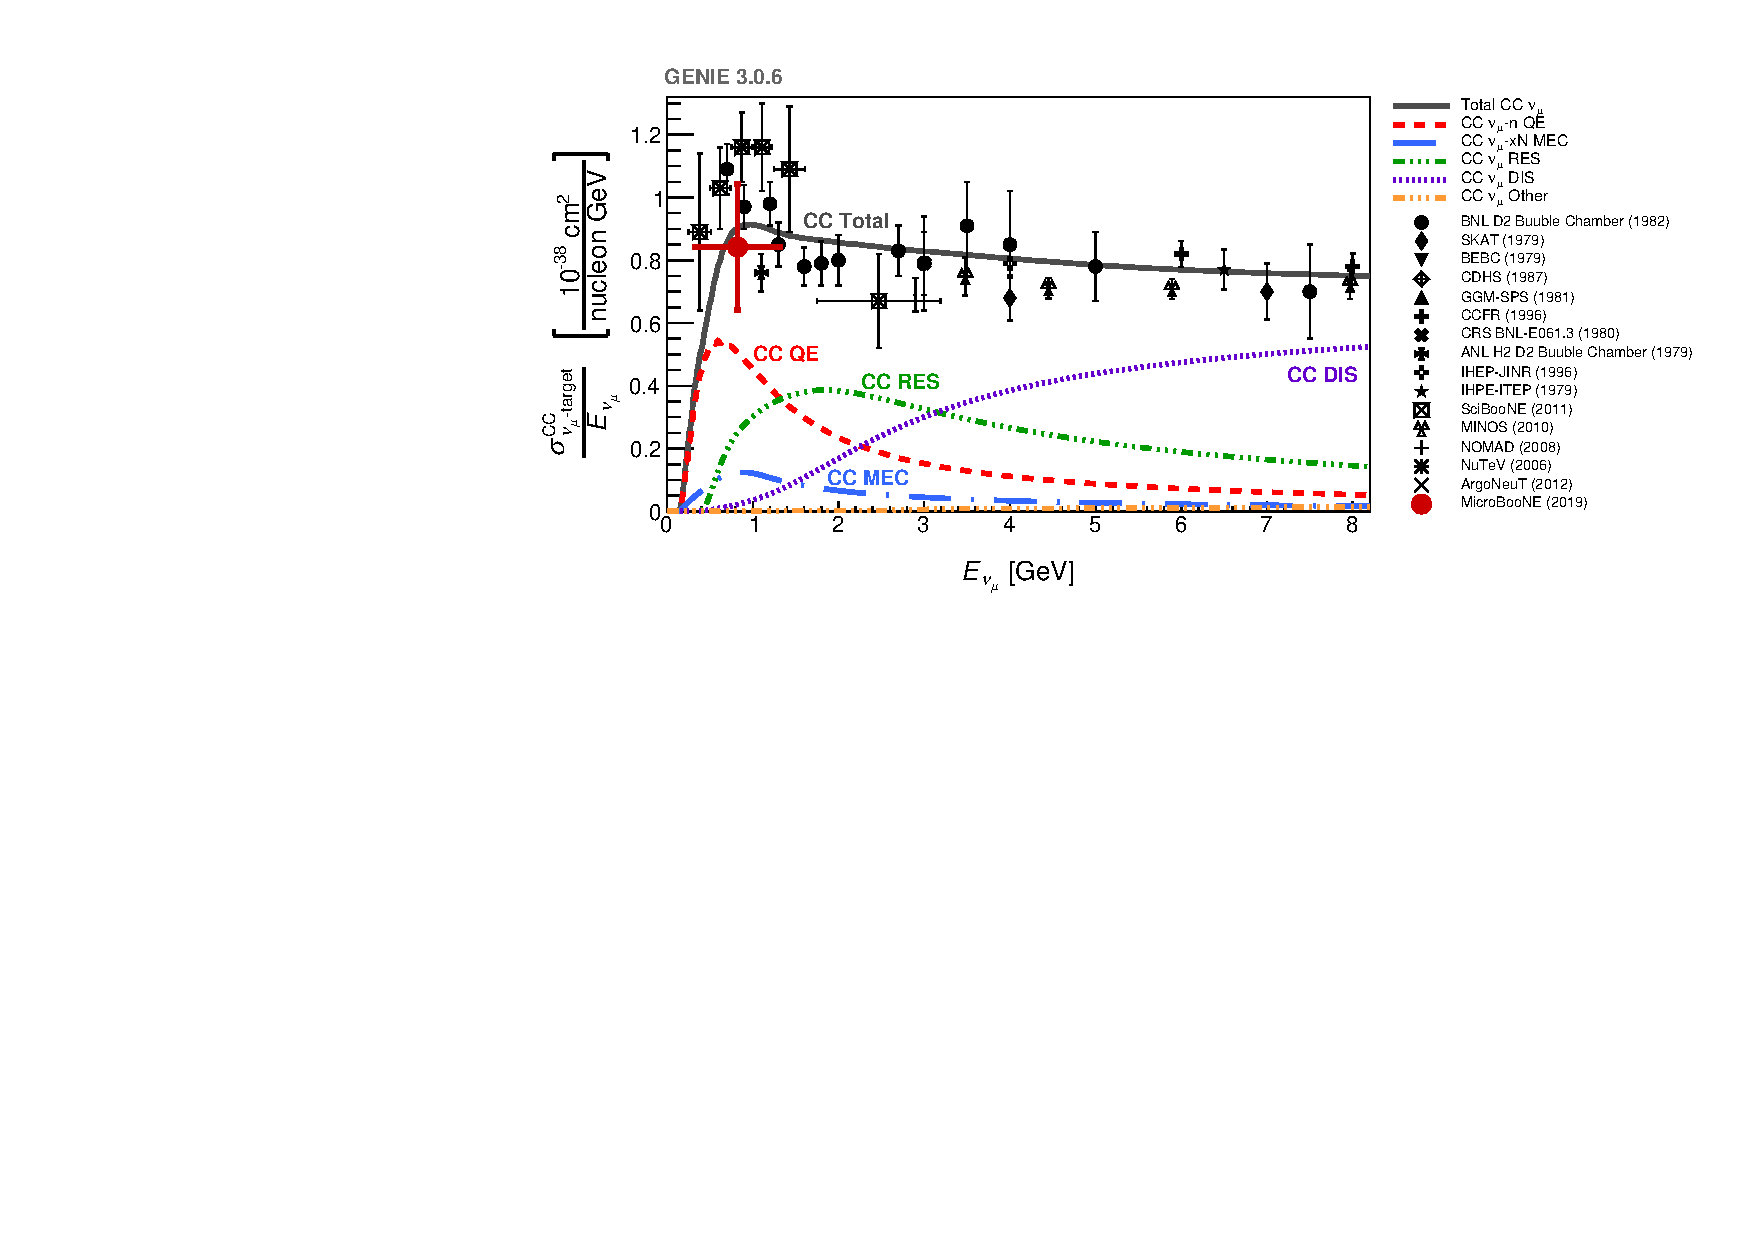
\includegraphics[width=.92\textwidth]{figures/xsec_Ev_numu_split.pdf}
%	    \vspace{-6.mm}
%	    \caption{}
%	    \label{inclusive_xsec_split}
%	\end{subfigure}
\vspace{-3mm}
	\caption[Inclusive Charged-Current Cross Section]{Total inclusive muon neutrino per-nucleon charged-current cross section divided by and as a function of the neutrino energy $E_{\nu_\mu}$ (solid black). %The neutrino energy scales for each contributing interaction process.
% The \acrshort{cc}\acrshort{qe} (dashed red) process is dominant for neutrino energies below $1.5$GeV. \acrshort{cc}\acrshort{mec} is shown in dashed-dotted blue. %\subref{inclusive_xsec} The \acrshort{res} (light and dark green dashed-three-dotted line) and \acrshort{dis} (light and dark purple dotted line) cross sections include interactions on neutrons and protons that are summed in \subref{inclusive_xsec_split}.
%    Further contributing processes are coherent scattering (yellow), neutrino-electron scattering (light brown) and neutrino interactions with sea-charm quarks in \acrshort{qe} and \acrshort{dis} channels (dark brown). %\subref{inclusive_xsec_split} Zoom of \subref{inclusive_xsec} for a neutrino energy range $[0,8.3] \ \text{GeV}$. Analogous plots for $\bar{\nu}_\mu$ can be found in \cref{xsec_Ev_numubar_log_legend} and \cref{xsec_Ev_numubar_legend} in appendix \ref{appendix_a}, respectively. 
    Data was kindly provided by G. Zeller \cite{Formaggio:2013kya}. The MicroBooNE data point is taken from \cite{DelTutto:2019cpu}.}
	\label{cc_inclusive_xsec_by_E}
\end{figure}
%
\vspace{-4mm}
\subsection{2p2h-Interactions and Nuclear Effects} \vspace{-2mm}\label{nuclear_effects}
%DUNE mean energy $2$GeV , 2p2h quite important
%Explain scattering processes and nuclear effects... introduce 2p2h and 2p2h models; explain reweighting and idea of going from one model to another by reweighting...
\iffalse%
\begin{figure}[H]
	\centering
	\includegraphics[width=.8\textwidth]{figures/MEC.pdf}
	\caption[]{}
	\label{MECs}
\end{figure}
\fi%
\iffalse%
\begin{figure}[H]
	\centering
	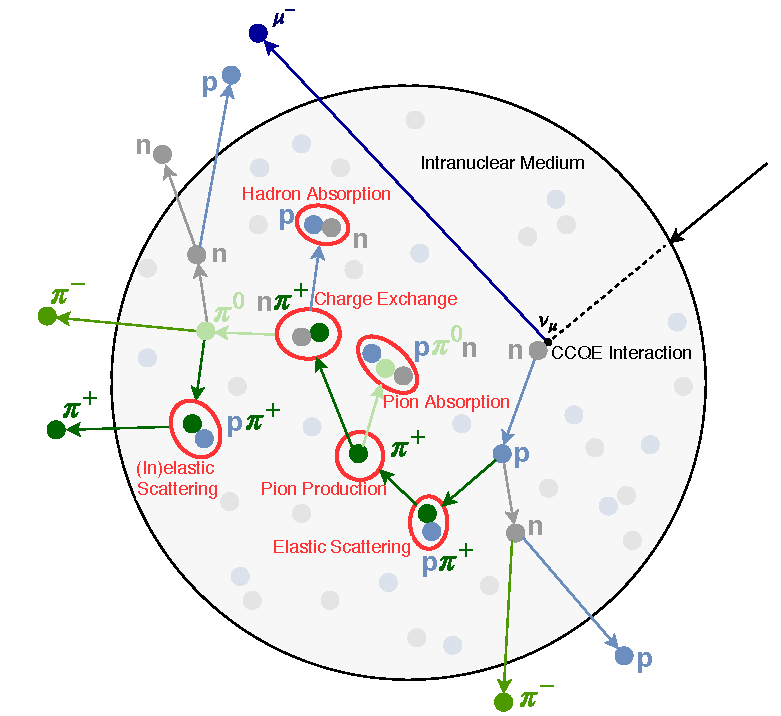
\includegraphics[width=.5\textwidth]{figures/FSIs.pdf}
	\caption[Illustration of Final-State Interactions]{Illustration of final-state interactions in an intranuclear cascade model approach. %The incoming muon neutrino $\nu_\mu$ represented by the black arrow followed by the dashed black line interacts via a charged-current quasi-elastic interaction with a neutron in an argon nucleus.
	%The outgoing muon (indigo line) and proton (light blue line) traverse the nuclear medium. The proton can undergo various types of hadronic FSIs such as (in)elastic scattering, pion production, hadron absorption and charge exchange. Pions in this figure are shown in dark green ($\pi^+$), regular green ($\pi^-$), and light green ($\pi^0$).
    }
	\label{FSIs}
\end{figure}
\fi%
%
    \begin{figure}[hbt]
	\centering
		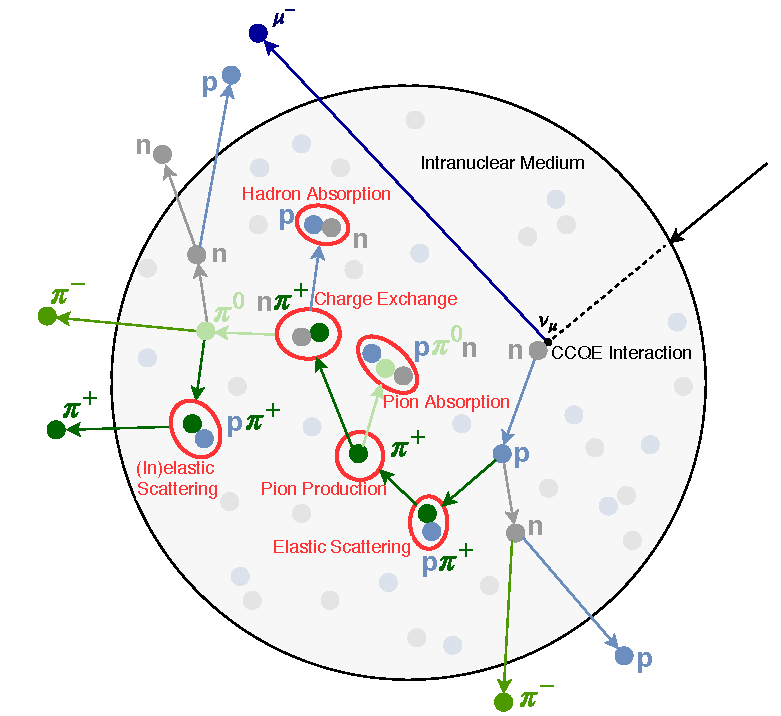
\includegraphics[width=0.45\textwidth]{figures/FSIs.pdf}
	\caption[Illustration of Final-State Interactions]{Final-State Interactions. %in an intranuclear cascade model approach. %The incoming muon neutrino $\nu_\mu$ represented by the black arrow followed by the dashed black line interacts via a charged-current quasi-elastic interaction with a neutron in an argon nucleus.
	%The outgoing muon (indigo line) and proton (light blue line) traverse the nuclear medium. The proton can undergo various types of hadronic FSIs such as (in)elastic scattering, pion production, hadron absorption and charge exchange. Pions in this figure are shown in dark green ($\pi^+$), regular green ($\pi^-$), and light green ($\pi^0$).
    }
	\vspace{4mm}
	\label{FSIs}
\end{figure}
%
Neutrino-nucleus interactions are processes in which the neutrino interacts with the nuclear target or its components depending on its energy. %Different neutrino interaction processes scale with the energy of the incident neutrino.
\iffalse%
\begin{figure}[htbp!]
	\begin{subfigure}[b]{.56\textwidth}
%		$\vcenter{\hbox{\includegraphics[width=\textwidth]{figures/2p2h_feynman_diagram.pdf}}}$
%		$\vcenter{\hbox{\includegraphics[width=\textwidth]{figures/2p2h-diagram.pdf}}\vspace{1.25cm}}$
		$\vcenter{\hbox{\includegraphics[width=\textwidth]{figures/2p2h-diagram2.pdf}}\vspace{1.25cm}}$
		\caption{}
		\label{mec_diagram}
	\end{subfigure}
	\begin{subfigure}[b]{.43\textwidth}
		$\vcenter{\hbox{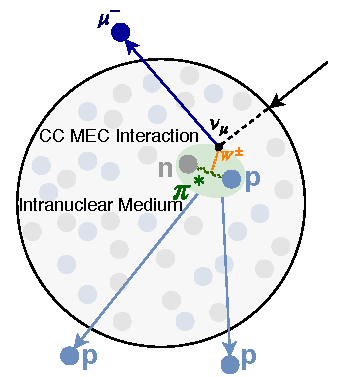
\includegraphics[width=\textwidth]{figures/CCMEC_nu_Ar.pdf}}}$
		\caption{}
		\label{mec_schematic}
	\end{subfigure}
	\caption[$2\text{p}$-$2\text{h}$ Scattering Process]{Illustration of the \acrlong{cc} $2\text{p}$-$2\text{h}$ scattering process: $\nu_\mu + 1\text{n}1\text{p} \rightarrow \mu^- + 2\text{p}$. \subref{mec_diagram} Feynman diagram of the $2\text{p}$-$2\text{h}$ interaction. In the absence of \acrshort{fsi}s, $2\text{p}$-$2\text{h}$ processes are all neutrino-nucleus interactions with two nucleons and no other hadrons in the final state. \subref{mec_schematic} Illustration of the $2\text{p}$-$2\text{h}$ process. Here, a pion-in-flight \acrshort{mec} gives rise to a neutrino $2\text{p}$-$2\text{h}$ interaction. The incoming muon neutrino $\nu_\mu$ (black arrow) interacts with two nucleons ($2\text{p}$, here one proton shown in light blue and one neutron shown in grey) bound by a virtual meson (here $\pi$-meson shown in green), that are kicked out of the nucleus, so that the remnant nucleus is left with two holes $2\text{h}$ in the final state. Hereby, the $\text{W}^-$ boson mediates an electroweak \acrshort{cc} quark flavor change, so that a muon (indigo arrow) is produced and the inital-state neutron becomes a final-state proton.}
	\label{mec}
\end{figure}
\fi%
%
    \begin{figure}[hbt]
    \centering
	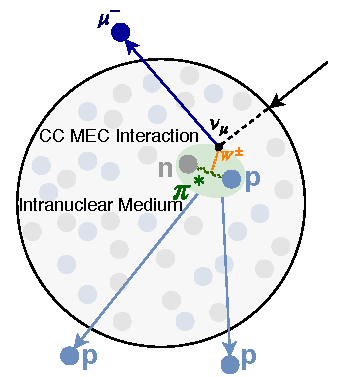
\includegraphics[width=0.45\textwidth]{figures/CCMEC_nu_Ar.pdf}
	\caption[Illustration of the \acrlong{cc} $2\text{p}$-$2\text{h}$ scattering process]{\acrshort{cc} \acrshort{2p2h} scattering% Here, a pion-in-flight \acrshort{mec} gives rise to a neutrino $2\text{p}$-$2\text{h}$ interaction
    .}
	\label{mec_schematic}
\end{figure}
%
While low-energy neutrinos may coherently scatter off the whole nucleus, neutrinos with higher incident energy may resolve the nucleus as a bound state of nucleons, single nucleons or quarks inside the nucleons \cite{Bathe-Peters:2022kkj}. %From lower to higher energies, the total inclusive neutrino interaction cross section scales for the partial \acrshort{cc}\acrshort{qe}, \acrshort{cc} \acrshort{2p2h}, \acrshort{cc}\acrshort{res}, \acrshort{cc}\acrshort{dis} and other \acrshort{cc} cross sections.
As shown in \cref{cc_inclusive_xsec_by_E}, different interaction processes are dominant at different energies \cite{bathe-peters:2020}. As \acrshort{dune} will operate at neutrino energies in the range of $0.5$ GeV up to $3.5$ GeV \cite{DUNE:2020ypp}, \acrshort{cc} \acrshort{2p2h} interactions make up one of the dominant neutrino interaction channels. %Neutrino interactions two-body interactions are complicated by nuclear effects due to short range correlations between nucleon in the nucleus
% from lower to higher energies we expect the cross section to be dominated in turn by \acrshort{cc}\acrshort{qe}, \acrshort{cc} \acrshort{2p2h}, \acrshort{cc}\acrshort{res}, and \acrshort{cc}\acrshort{dis} interactions.
%As there are many different neutrino interaction processes contributing to the total cross section, these interaction processes have a strong influence on the totatl neutrino-nucleus cross section, so that the understanding of neutrino-nucleus scattering becomes already complex.
Theoretical predictions are further complilcated by nuclear effects. These can be categorised into intitial-state effects, multinucleon-correlation effects and \acrlong{fsi}s (\acrshort{fsi}s). %The whole picture of a neutrino nucleus-interaction 
\acrshort{fsi}s in a neutrino-nucleus interaction are illustrated by the schematic in \cref{FSIs}.
%
The most relevant nuclear effects for the analysis presented in this report are \acrshort{fsi}s as well as $2$-body currents in the initial nuclear state arising from $2$ nucleons bound by the exchange of a virtual meson, referred to as \acrlong{mec}s (\acrshort{mec}s). The formation of nucleons into such bound states inside the nucleus enables the neutrino to scatter off bound states of two (or more) nucleons giving raise to \acrshort{2p2h} interactions (see \cref{mec_schematic}). In the absence of \acrshort{fsi}s, the \acrshort{2p2h} interaction is a neutrino interaction on two particles leaving two holes inside the nucleus. 
%The importance of these multi-nucleon channels was first pointed out in \cite{Martini:2009uj} as these processes are considered to contribute to the most significant part of cross-section uncertainties \cite{Niewczas:2019fro}.
Clarifying the degree to which it can be distinguished from look-alike processes \cite{PhysRevC.98.045502} in argon and to have the ability to correctly account for uncertainties from differences between models is therefore of substantial interest. For example, as \acrshort{fsi}s may lead to the absorption of one of the two final-state nucleons, it can be experimentally very challenging to distinguish \acrshort{2p2h} from \acrshort{cc}\acrshort{qe} interactions. %Since \acrshort{fsi}s can obscure the nature of the primary neutrino interaction and hence complicate the neutrino energy reconstruction, the understanding of \acrshort{fsi}s is crucial for neutrino physics analyses.
A particular set of \acrfull{tki} variables \cite{Lu:2018stk} is especially sensitive to nuclear effects. %The vector transverse momentum imbalance 
%
%\begin{align} \label{dpt}
%    \delta \vec{p}_T = \vec{p}^{\hspace{.2ex} \text{T}}_{\ell'} + \vec{p}^{\hspace{.2ex} \text{T}}_{h'}
%\end{align}
%
%is the sum of the projections of the lepton and hadron momenta onto the plane transverse with respect to the incoming neutrino direction. 
The transverse angular imbalance $\delta\alpha_\text{T} \equiv \text{arccos}\left(\frac{-\vec{p}_{\ell'}^{\hspace{.2ex} \text{T}} \cdot \vec{p}_{\text{h}'}^{\hspace{.2ex} \text{T}}}{p_{\ell'}^\text{T}p_{\text{h}'}^\text{T}}\right)$
%$\delta\alpha_\text{T} \equiv \text{arccos}\left((-\vec{p}_{\ell'}^{\hspace{.2ex}} \text{T} \cdot \vec{p}_{\text{h}'}^{\hspace{.2ex} \text{T}})/(p_{\ell'}^\text{T}p_{\text{h}'}^\text{T})\right)$
%
%\begin{align} \label{dat}
%    \delta\alpha_\text{T} &\equiv \text{arccos}\left(\frac{-\vec{p}_{\ell'}^{\hspace{.2ex} \text{T}} \cdot \vec{p}_{\text{h}'}^{\hspace{.2ex} \text{T}}}{p_{\ell'}^\text{T}p_{\text{h}'}^\text{T}}\right)
%\end{align}
%
gives information about the direction of the transverse momentum imbalance and to what extent the final state of the neutrino-nucleus interaction is transversely accelerated $(|\vec{p}_{\text{h}'}^{\hspace{.2ex} \text{T}}|
< |\vec{p}^{\hspace{.2ex} \text{T}}_{\ell'}| \ \text{and} \ \delta\alpha_\text{T} < 90^\circ)$ or decelerated
$(|\vec{p}_{\text{h}'}^{\hspace{.2ex} \text{T}}|
> |\vec{p}^{\hspace{.2ex} \text{T}}_{\ell'}| \ \text{and} \ \delta\alpha_\text{T} > 90^\circ)$ 
by nuclear effects causing the TKI~\cite{Lu:2018stk}.

% Description of specific apparatus you have used, if appropriate. Do not describe general apparatus, e.g. the entire ATLAS detector.
\vspace{-4mm}
\section{Investigating model differences with \texorpdfstring{\acrshort{dune}}{TEXT}} \vspace{-3mm} \label{dune_measurement}
%Briefly describe DUNE and why it is good for measuring 2p2h cross sections...
%
In order to theoretically predict and experimentally understand data associated with neutrino-nucleus cross sections, the \acrshort{genie} neutrino event generator performs simulations of neutrino interactions according to underlying theoretical models. A number of novel parameters have been implemented to allow new degrees of freedom in the uncertainty model. In the future, these parameters will be constrained by fitting them to experimental data, ultimately giving rise to a GENIE theory-driven uncertainty model. % The hoped outcome is a better simulation-data agreement with improved uncertainties based on the fit.
This will provide sufficient freedom in the \acrshort{dune} model to fit the eventual data without bias \cite{PhysRevD.105.072001}.

\vspace{-3mm}
%\subsection{Event Reweighting}
\subsection{Propagating Uncertainties} \vspace{-2mm}
%Any nominal \acrfull{mc} prediction $P$ such as a physical parameter (e.g. axial mass) or a function of a kinematical parameter (e.g. a cross section as a function of energy) as a neutrino-generator input physics quantity cannot be easily expressed analytically or tabulated. 
Since it is too costly in terms of time and resources to (re)generate \acrshort{mc} simulations for every change in every parameter, evaluating uncertainties via reweighting is more feasible to vary parameters, e.g. in a fit to data.
In order to deal with uncertainties associated with a \acrfull{mc} predicted physical parameter $P$, a systematic parameter $x_P$ is introduced, such that one can formulate a problem in terms of $x_P$ and evaluate an event weight as a function of $x_P$. Tweaking $x_P$ may then modify the corresponding $P$ with estimated standard deviation $\delta P$ as \cite{Andreopoulos:2009rq}
\vspace{-3mm}%
\begin{align} \label{tweak_parameters}
    P \longrightarrow P' = P\left( 1 + x_P \frac{\delta P}{P} \right) \ .
\end{align}
%
Setting $x_P=0$ leaves $P$ unchanged from its nominal value. Tweaking the $x_P$ by $\pm 1$ modifies the associated $P$ by $\pm \delta P$.
%\subsection{Propagating Uncertainties}
When propagating neutrino-nucleus cross-section uncertainties, the neutrino interaction probability is modified directly. Therefore, it is nearly independent on the details of the physics modeling. To evaluate an event rate, one calculates the ratio between the nominal differential cross section $\frac{\text{d}^n\sigma}{\text{d}K^n}$ and the differential cross section $\frac{\text{d}^n\sigma'}{\text{d}K^n}$ computed using the modified input physics parameters evaluated at the kinematical phase space $\{K^n\}$ \cite{Andreopoulos:2009rq}:
\vspace{-3mm}%
\begin{align} \label{event_weight}
%    w_\sigma = \frac{\frac{\text{d}^n\sigma}{\text{d}K^n}}{\frac{\text{d}^n\sigma'}{\text{d}K^n}}
    w_\sigma = \frac{\text{d}^n\sigma}{\text{d}K^n} \bigg/ \frac{\text{d}^n\sigma'}{\text{d}K^n}
\end{align}
\vspace{-3mm}%

%describe Reweight here...

% Description of your work and summary of results
\vspace{-9mm}
\section{Analysis and Results} \vspace{-3mm}
%Describe plots of chosen variables from plotting script... show GENIEReweight plots, explain them...; what can we get out of them?...
%Can area-normalise plots in geniev3plottingscript in worst case scenario
In order to interpret data, studies of accelerator neutrinos rely on detailed simulations of beam production, neutrino scattering, final-state particle transport and the detector response. Neutrino event generators such as \acrshort{genie} have models of neutrino cross sections implemented. %However, due to the lack of a comprehensive theoretical framework that can predict all observables for all interaction modes, the current approach for neutrino event generators is to adopt a factorisation scheme in which model components are joined together to fully simulate the scattering process. In that manner, the simulation of a typical neutrino-nucleus scattering event first involves the interaction mode and initial particle kinematics. Then, outgoing kinematics for the final-state particles are chosen according to the differential cross section appropriate for the sampled interaction mode. The event simulation finishes after considering intranuclear rescattering of the outgoing hadrons using a \acrshort{fsi} model. \cite{Bathe-Peters:2022kkj}
For the results shown in this report, I used \acrshort{genie} v$3.4.0$ with different model configurations. In all configurations, a \acrfull{lfg} model is used to describe the nuclear ground state prior to the neutrino interaction. % In the $\verb!G18_10a!$ model set, \acrshort{cc}\acrshort{qe} and \acrshort{2p2h} scattering are simulated using the $1$p$1$h and \acrshort{2p2h} Valencia model, respectively. Long-range nucleon-nucleon correlations are accounted for in this model via the \acrfull{rpa}. Resonance and coherent pion production are modeled by the Berger and Sehgal model \cite{Berger:2008xs}. The Bodek and Yang model \cite{Bodek:2002vp} is used for \acrshort{dis} and \acrshort{fsi}s are simulated using an intranuclear cascade model called $hA2018$ \cite{Dytman2021}. 
For this analysis, the most important difference when considering the results shown below is to consider the three different \acrshort{2p2h} models used to simulate \acrshort{2p2h} scattering. These are the Empirical, Valencia and SuSAv$2$ \acrshort{cc} \acrshort{2p2h} models, whereby the latter one is intended to be the default model for \acrshort{dune}. The goal is to develop reweighting parameters that will go from the SuSAv$2$ model to predictions from other models.
%While the $\verb!G18_01a!$ model set uses the GENIE Empirical \acrshort{cc} \acrshort{2p2h} model, the $\verb!G18_10a!$ model set employs the Valencia \acrshort{cc} \acrshort{2p2h} model. The remaining model configuations use the SuSAv$2$ \acrshort{cc} \acrshort{2p2h} model.

%\subsection{Comparison of Models}
%In the following three different sets of plots are shown. The first set of plots in \cref{set1} shows effects of \acrshort{fsi}s on chosen variable distributions. 
%In the second set of plots in \cref{set2}, the current \acrshort{cc} \acrshort{2p2h} models being implemented in the neutrino event generator GENIE are compared and differences that allow possible discrimination between the models are highlighted. 
%The systematic parameters described in \cref{systematic_parameters} are evaluated in \cref{set3}.
\vspace{-3mm}
\subsection{CC 2p-2h Model Comparisons} \label{set2} \vspace{-2mm}
%3 models postFSI (according to equally likely data, phase space that is covered by reasonable models that we want to cover by uncertainties-> uncertainties)
Due to insufficient \acrshort{mc}-data agreement for the current \acrshort{cc} \acrshort{2p2h} models, one has to account for differences between these models in associated uncertainties. The set of plots in \cref{set2_plots} provides a direct comparison and highlights possible discrimination between the available \acrshort{cc} \acrshort{2p2h} models at present in GENIE.
%\vspace{-2mm}%
\begin{figure}[htb!]
	\begin{subfigure}[b]{.325\textwidth}
%        \includegraphics[width=\textwidth]{figures/1DComp_ErecAbsBias_14_ccmec.pdf}
        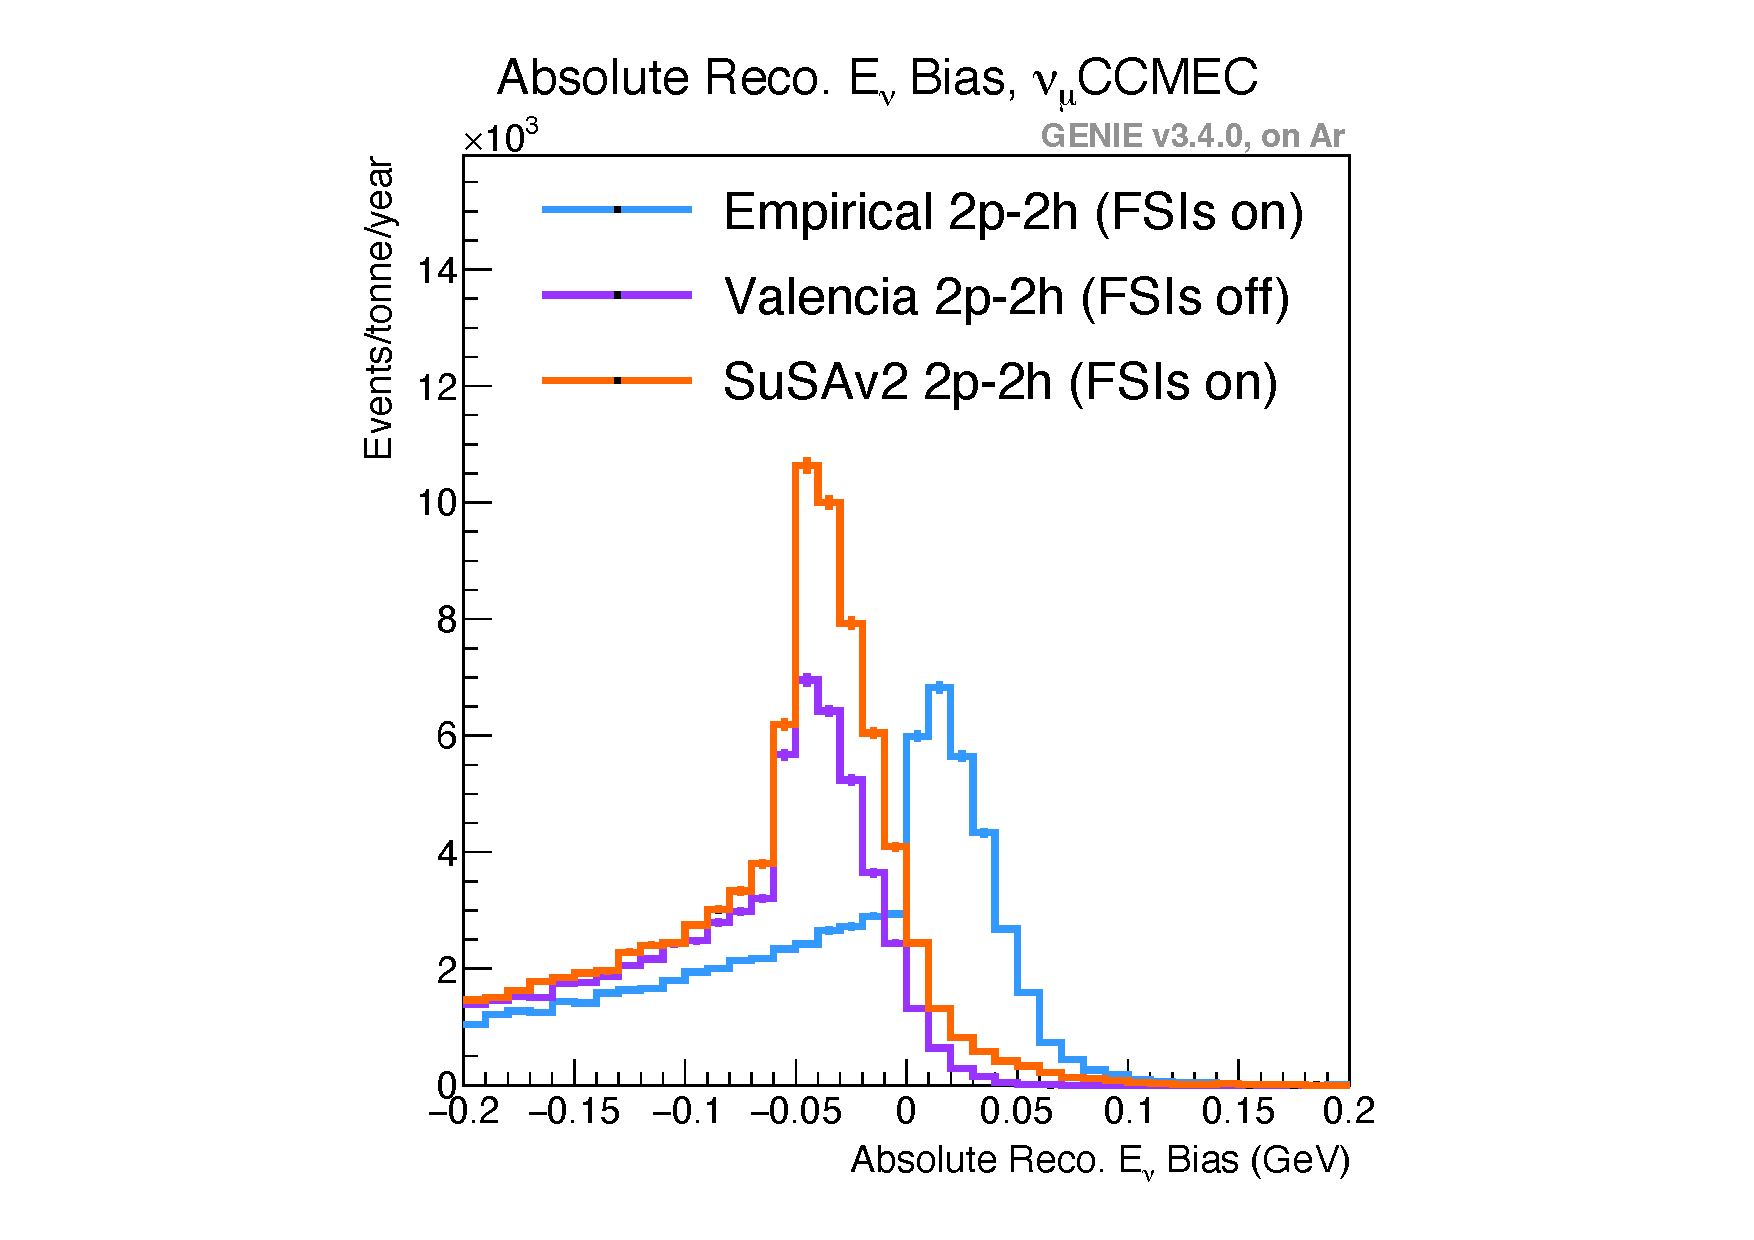
\includegraphics[width=\textwidth]{figures/postFSIs/1DComp_ErecAbsBias_14_ccmec_edited.pdf}
%        \vspace{-2.mm}
% \caption{}
	\label{set2_a}
    \end{subfigure}
	\begin{subfigure}[b]{.305\textwidth}
%        \includegraphics[width=\textwidth]{figures/1DComp_ErecRelBias_14_ccmec.pdf}
        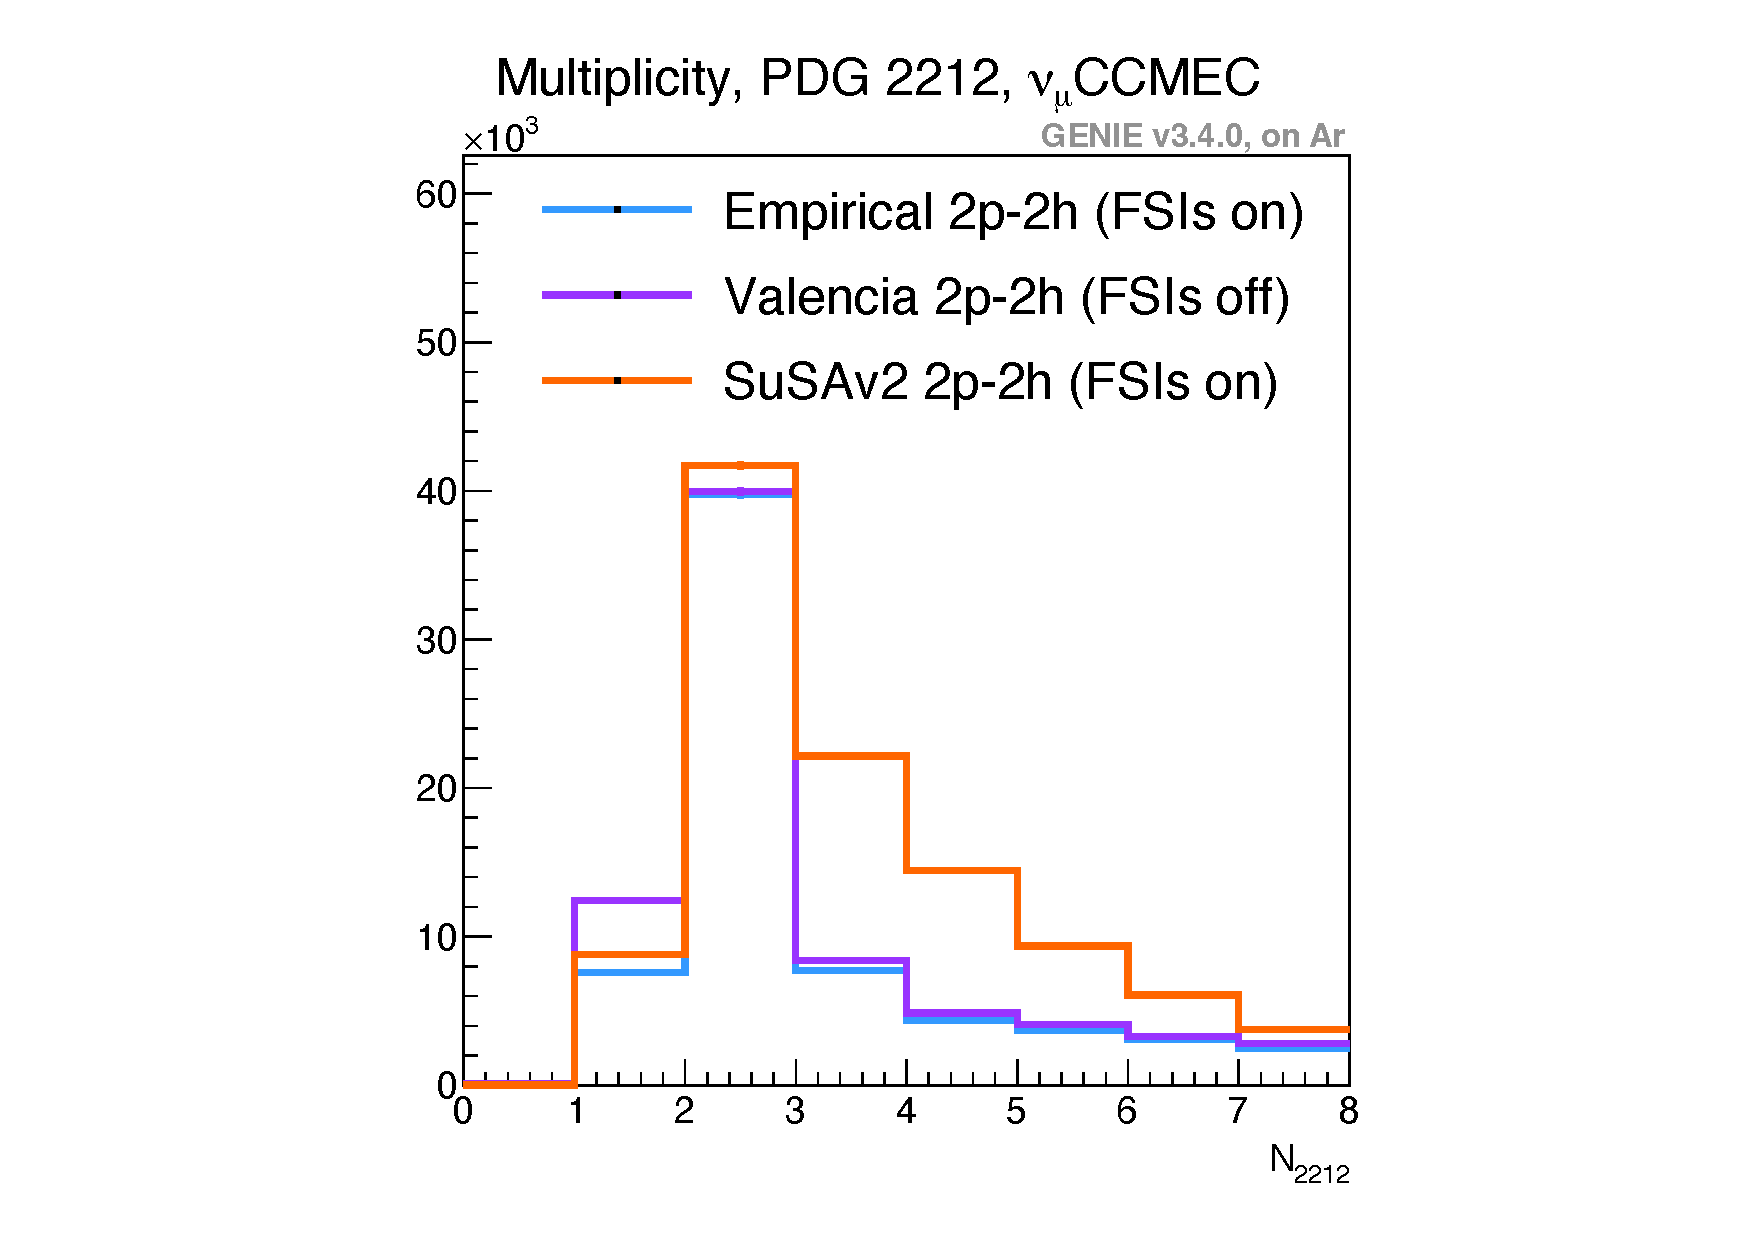
\includegraphics[width=\textwidth]{figures/postFSIs/1DComp_mult_2212_14_ccmec_multp_edited.pdf}
%        \vspace{-2.mm}
%    \caption{}
	\label{set2_b}
    \end{subfigure}
     %\vspace{-8mm}
 \begin{subfigure}[b]{.325\textwidth}
%        \includegraphics[width=\textwidth]{figures/1DComp_ErecAbsBias_14_ccmec.pdf}
        %
\includegraphics[width=\textwidth]{figures/postFSIs/1DComp_LeadP_p_14_ccmec_edited.pdf}
        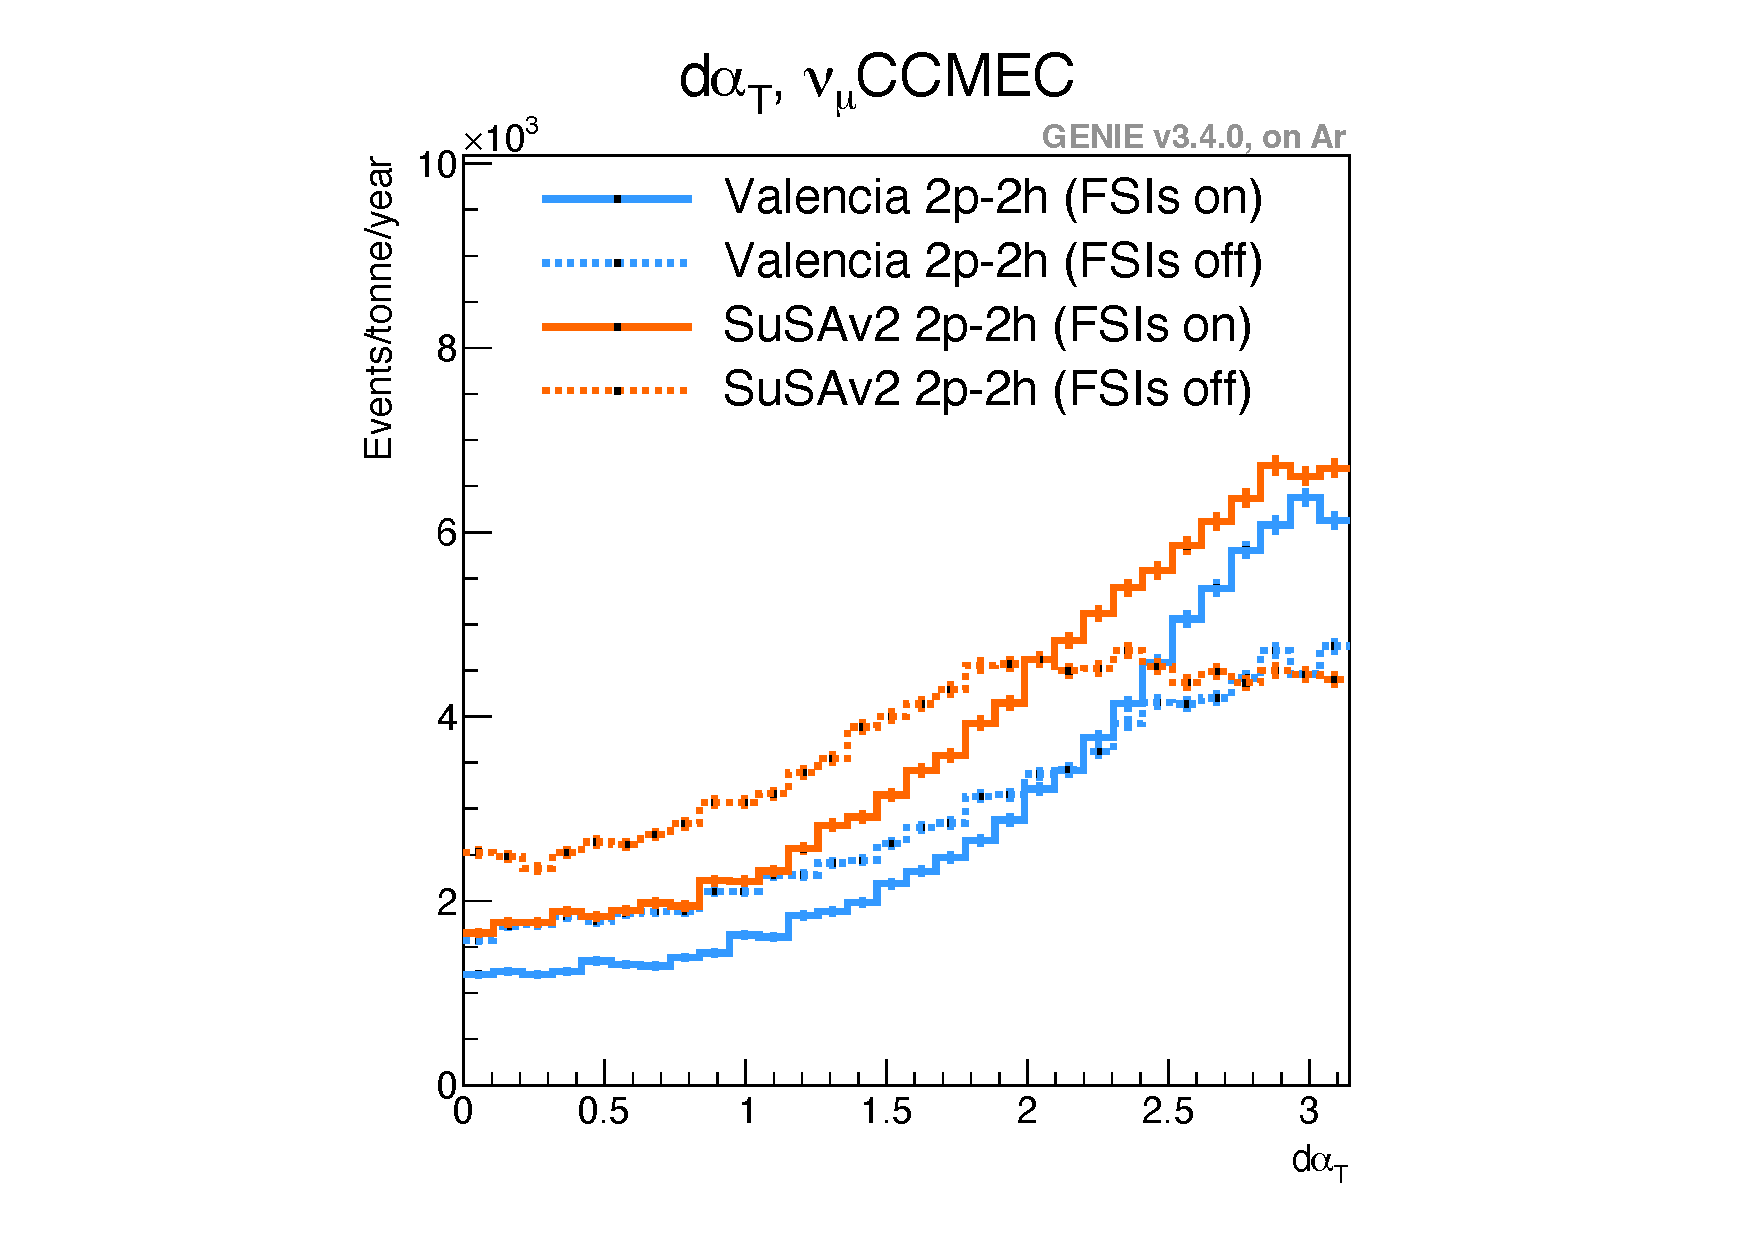
\includegraphics[width=\textwidth]{figures/FSI_vs_noFSI/1DComp_dat_14_ccmec.pdf}
%        \vspace{-6.mm}
%    \vspace{-2mm}
%	\caption{}
	\label{set2_c}
    \end{subfigure}
    \vspace{-6mm}
	\caption[]{Distributions of the number of events of GENIE-generated muon neutrino CC interactions on argon as a function of (left) the absolute reconstructed neutrino energy bias, (middle) the proton multiplicity and (right) the leading proton momentum.\vspace{-2mm}}
	\label{set2_plots}
\end{figure}
\vspace{-1mm}%
In \cref{set2_plots} (left), one can observe a clear separation between the distributions of the Empirical and SuSAv2 \acrshort{cc} \acrshort{2p2h} models. Considering the neutrino energy bias $E_\nu = E_\text{reco} - E_\text{true}$ in an experiment like DUNE gives insight on choosing the right uncertainty model, such that the measurement of the oscillation parameters is not biased in case the wrong model is chosen, in which case nature could be closer to one of the other models. Regarding the proton multiplicity shown in \cref{set2_plots} (middle), while the Empirical and Valencia model make rather similar predictions, the SuSAv2 model stands out in a way that could be potentially observed in an experiment like \acrshort{dune}. %One can also observe differences in the leading proton momentum distribution in \cref{set2_c} between the three models.
\vspace{-3mm}
\subsection{Impact of Final-State Interactions}  \vspace{-2mm} \label{set1}
%3 different sets of plots: comparison preFSI and postFSI and comment on what FSI (difference, effect of FSIs) was:

%In order to understand neutrino interactions inside oscillation experiments, the interaction target must be carefully chosen. Interactions on any target material that is not hydrogen will lead the final-state of a neutrino interactions to be subject to nuclear effects, in particular \acrshort{fsi}s, as described in \cref{nuclear_effects}. In order to demonstrate the effects of \acrshort{fsi}s on chosen variable distributions,
Fig. \ref{set2_plots} (right) illustrates how \acrshort{fsi}s can contribute to the alteration of the final state of a neutrino interaction. 
%This is also to demonstrate the effects of \acrshort{fsi}s and their importance in understanding the final-state of a neutrino-nucleus interaction on argon.
The impact of \acrshort{fsi}s is particularly significant in \acrshort{dune} because argon as a relatively large nucleus is used as the neutrino-nucleus interaction target. The $\mathrm{d}\alpha_T$ distributions in \cref{set2_plots} (right) are comparisons between the Valencia and SuSAv$2$ \acrshort{cc} \acrshort{2p2h} models in the pre- and post-FSI scenarios. 
\iffalse%
\begin{figure}[htb!]
	\begin{subfigure}[b]{.32\textwidth}
        \includegraphics[width=\textwidth]{figures/FSI_vs_noFSI/1DComp_dpt_14_ccmec.pdf}
        %\includegraphics[width=\textwidth]{figures/FSI_vs_noFSI/1DComp_LeadP_p_14_ccmec.pdf}
%        \vspace{-6.mm}
	\caption{}
	\label{set1_a}
    \end{subfigure}
	\begin{subfigure}[b]{.32\textwidth}
        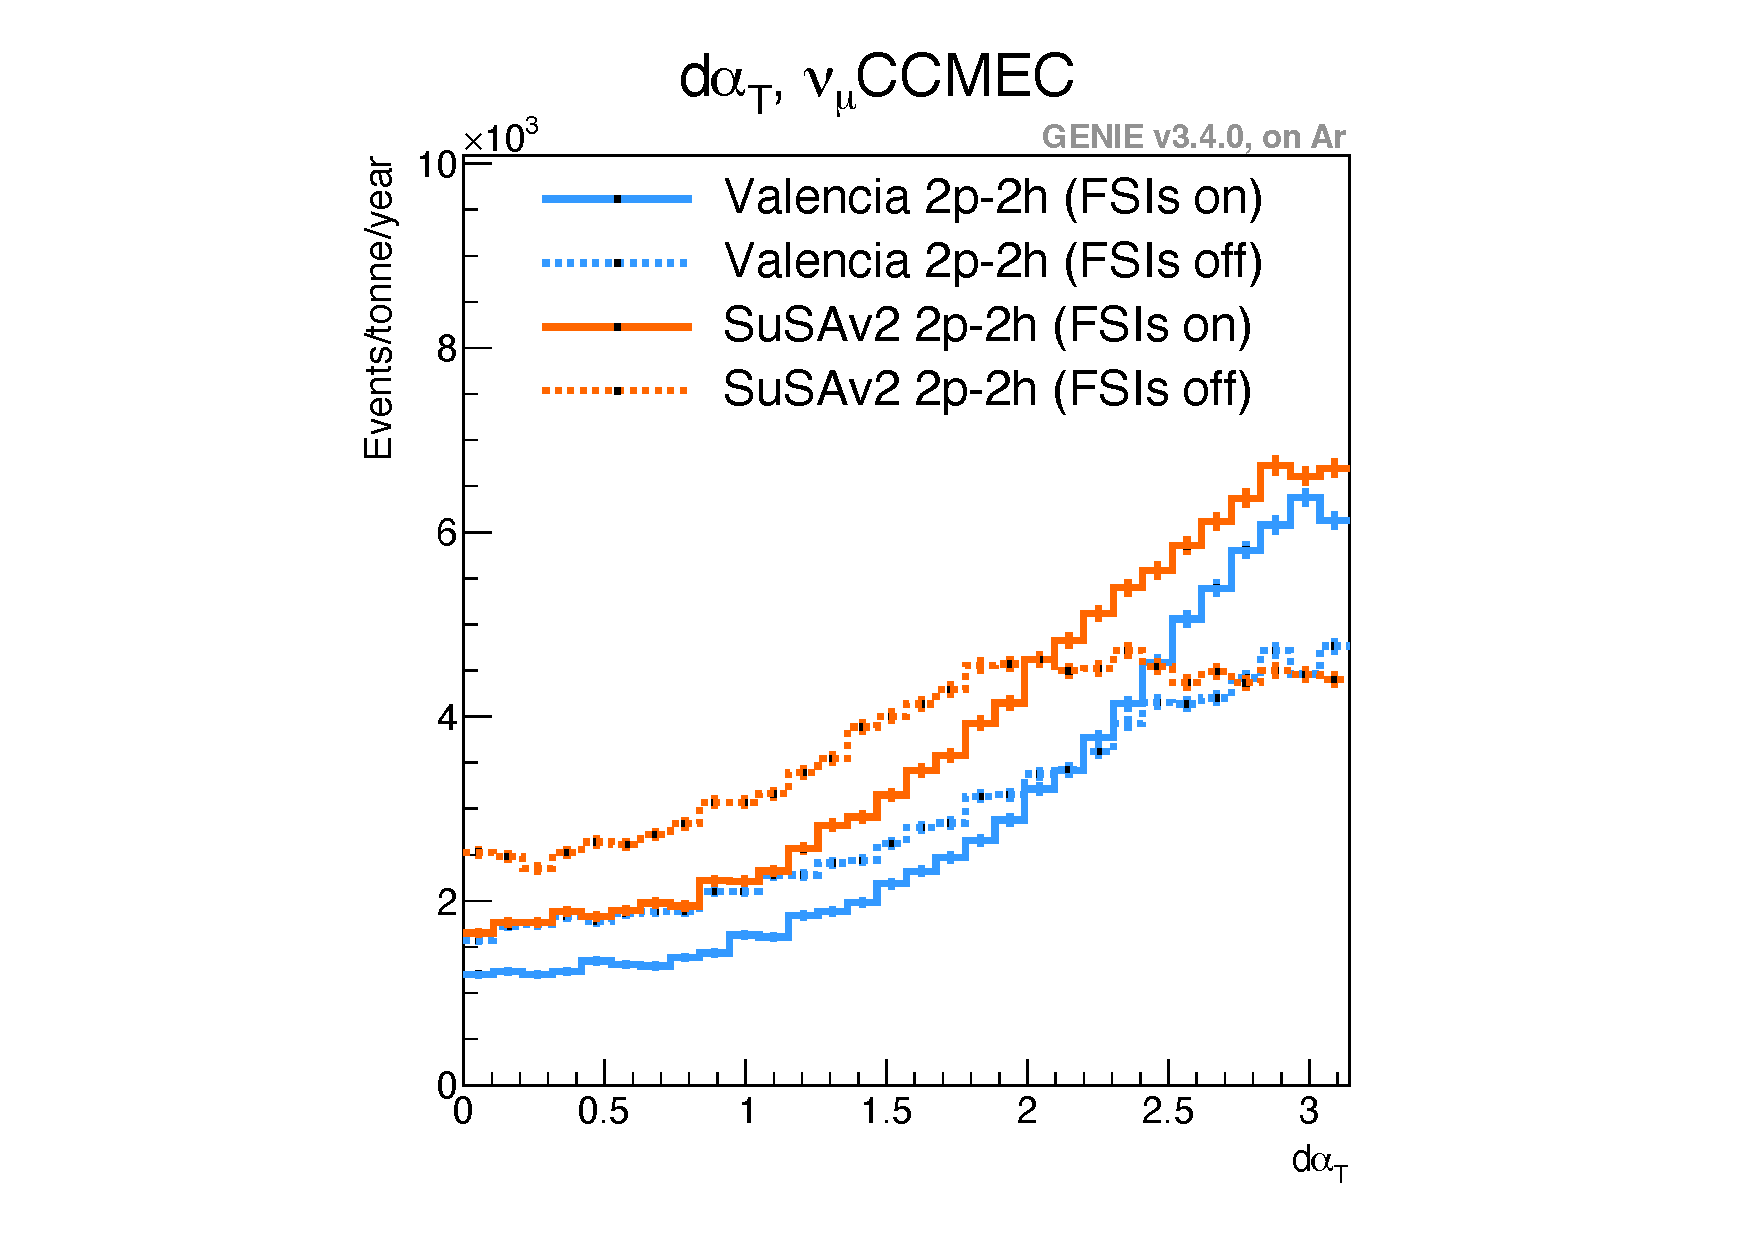
\includegraphics[width=\textwidth]{figures/FSI_vs_noFSI/1DComp_dat_14_ccmec.pdf}
%        \vspace{-6.mm}
	\caption{}
	\label{set1_b}
    \end{subfigure}
	\begin{subfigure}[b]{.32\textwidth}
        \includegraphics[width=\textwidth]{figures/FSI_vs_noFSI/1DComp_DecayAngMECNP_14_ccmec.pdf}
%        \vspace{-6.mm}
	\caption{}
	\label{set1_c}
    \end{subfigure}
	\caption[]{Distributions of the number of events of muon neutrino CC interactions on argon for the GENIE neutrino event generator as a function of (\subref{set1_a}) $\delta p_\text{T}$ , (\subref{set1_b}) $\delta \alpha_\text{T}$ and (\subref{set1_c}) the decay angle of the final-state nucleon pair in its rest frame.}
	\label{set1_plots}
\end{figure}
\fi%
%As \acrshort{fsi}s can cause the final-state hadron to loose momentum by intranuclear rescattering on the way out of the nucleus, they can cause more relative events in the peak region ot the $dp_T$ variable distribution in \cref{set1_a}. This effect is accounted for more strongly for the \acrshort{cc} \acrshort{2p2h} SuSAv$2$ model.
In the absence of nuclear effects, the $\mathrm{d}\alpha_T$ distribution in \cref{set2_plots} (middle) is close to a uniform distribution. Due to protons that were strongly decelerated in the transverse plane by \acrshort{fsi}s, one observes an asymmetry in the $\mathrm{d}\alpha_T$ variable with the introduction of \acrshort{fsi}s. %The scattering angle between the struck nucleon pair in \cref{set2_plots} (right) features the most significant differences in both the Valencia and SuSAv$2$ models when comparing the cases of pre- vs. post-FSI scenarios.
\vspace{-3mm}
\subsection{New Systematic Uncertainty Parameters} \vspace{-2mm}\label{set3}
%Reweighting plots (Norm, shape ..., maybe show one hadron and muon variable, only if measure muon or proton can measure difference, PN dials apply to hadronic side, able to measure it in DUNE)
%energy bias plot, Proton KE or leading momentum, lepton momentum easy to measure, multiplicity proton,
%\subsection{Parameter Dials} \label{systematic_parameters}
In the following, I am introducing new parameters, also known as 'dials', to account for uncertainties in \acrshort{cc} \acrshort{2p2h} interactions that arise not only in the SuSAv$2$ model used, but also from differences between the \acrshort{cc} \acrshort{2p2h} models. These parameters were adapted from \cite{PhysRevD.105.072001} for \acrshort{dune}, in which the base model was changed to the SuSAv$2$ model. The following plots were generated using GENIEReweight and show the tweaking of four systematic parameters, i.e. $\verb!NormCCMEC!$ (\cref{normccmec}), $\verb!DecayAngMEC!$ (\cref{decayangmec}), $\verb!FracPN_CCMEC!$ (\cref{fracpnccmec_plots}) and $\verb!XSecShape_CCMEC!$ (\cref{xsecshapeccmec}).
\vspace{-8mm}
\paragraph{NormCCMEC}
The $\verb!NormCCMEC!$ parameter changes the overall absolute normalisation of the \acrshort{cc} \acrshort{2p2h} cross section. This parameter sets the alterations to the strength of the untuned \acrshort{cc} \acrshort{2p2h} cross section calculated via reweighting \cite{PhysRevD.105.072001}. A parameter value of $0$ corresponds to the default normalisation of \acrshort{cc} \acrshort{2p2h} interactions in GENIE. Setting a positive value increases the average cross section, whereas a negative value decreases it (see \cref{normccmec}).
%
%\vspace{-2mm}%
\begin{figure}[htb!]
	\begin{subfigure}[b]{.33\textwidth}
%        \includegraphics[width=\textwidth]{figures/Norm_CCMEC/1DComp_cosThetaLep_14_ccmec.pdf}
        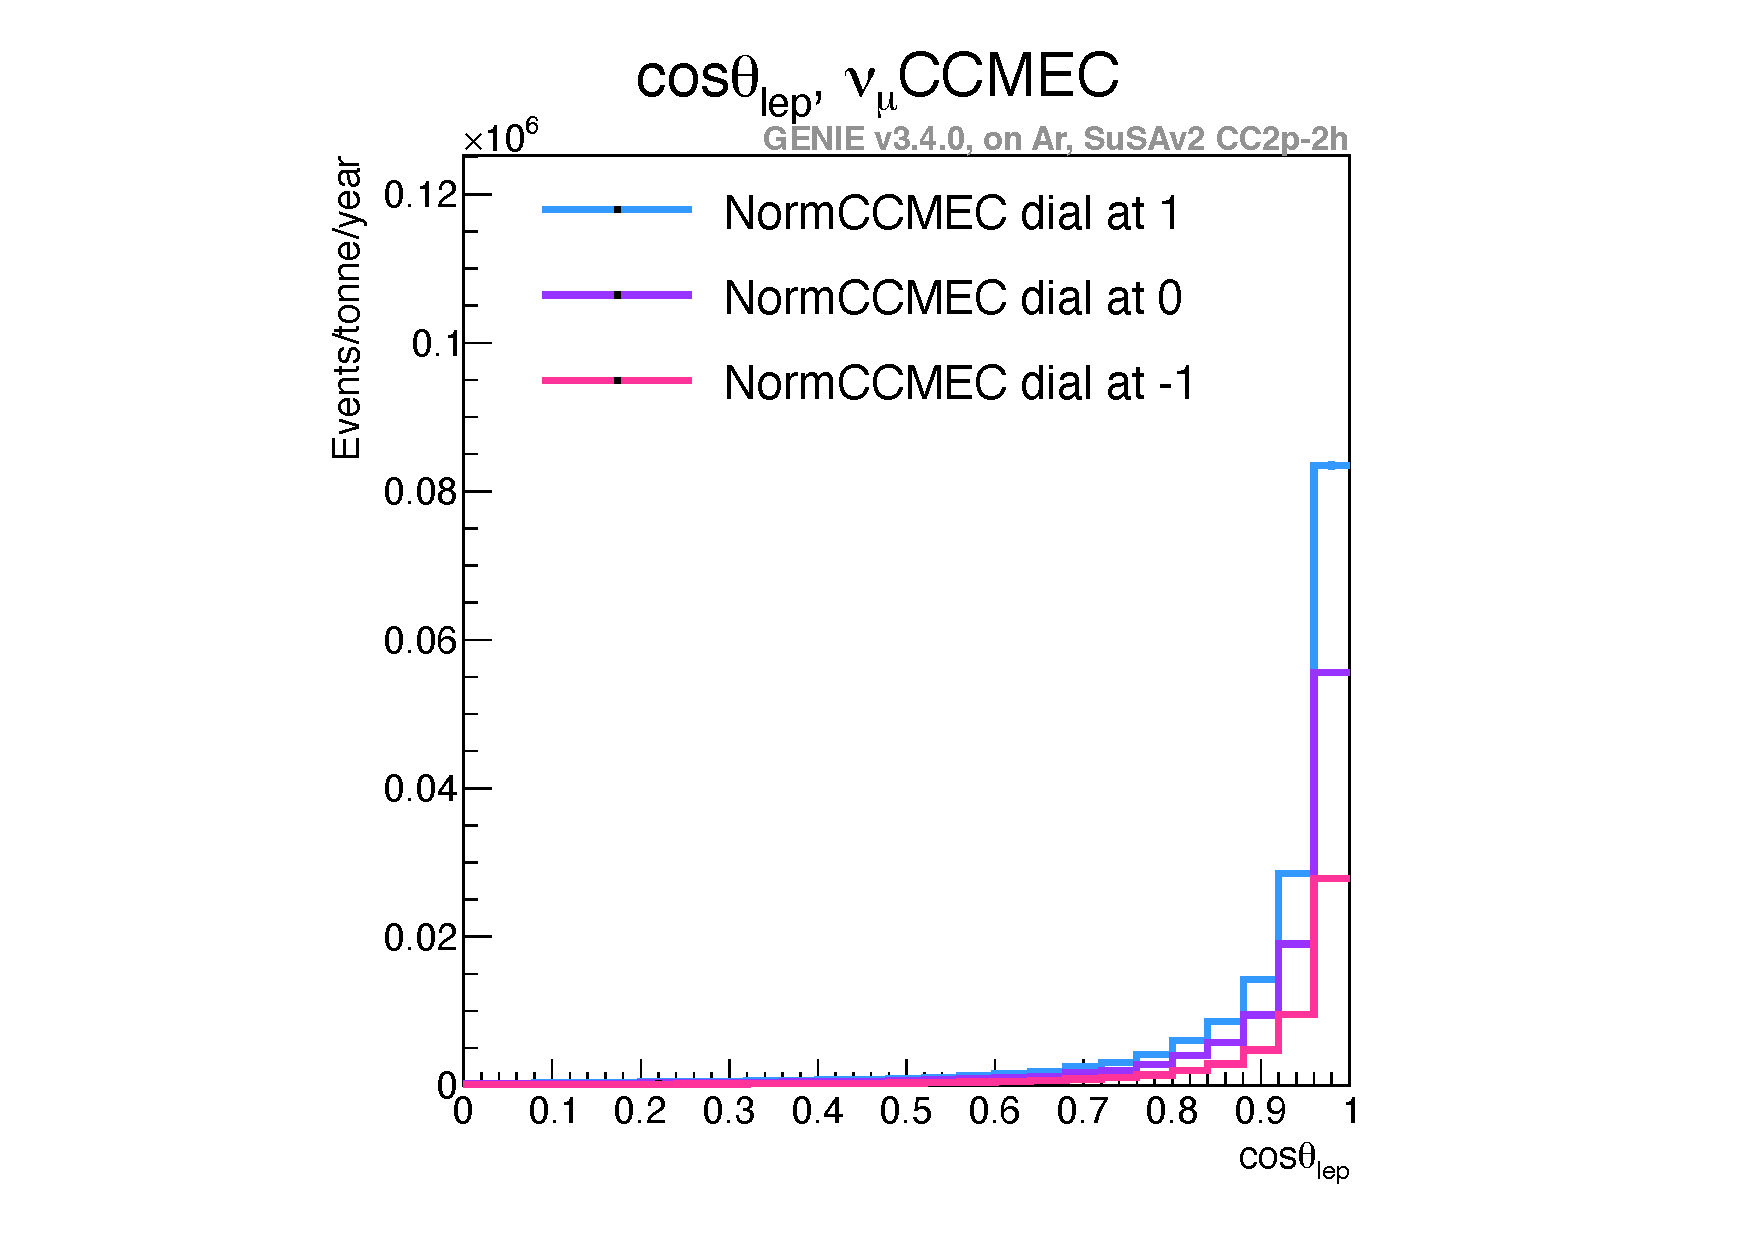
\includegraphics[width=\textwidth]{figures/Norm_CCMEC/1DComp_cosThetaLep_14_ccmec_edited.pdf}
%        \vspace{-6.mm}
%	\caption{}
	\label{normccmec_a}
    \end{subfigure}
	\begin{subfigure}[b]{.32\textwidth}
%        \includegraphics[width=\textwidth]{figures/Norm_CCMEC/1DComp_LeadP_p_14_ccmec.pdf}
        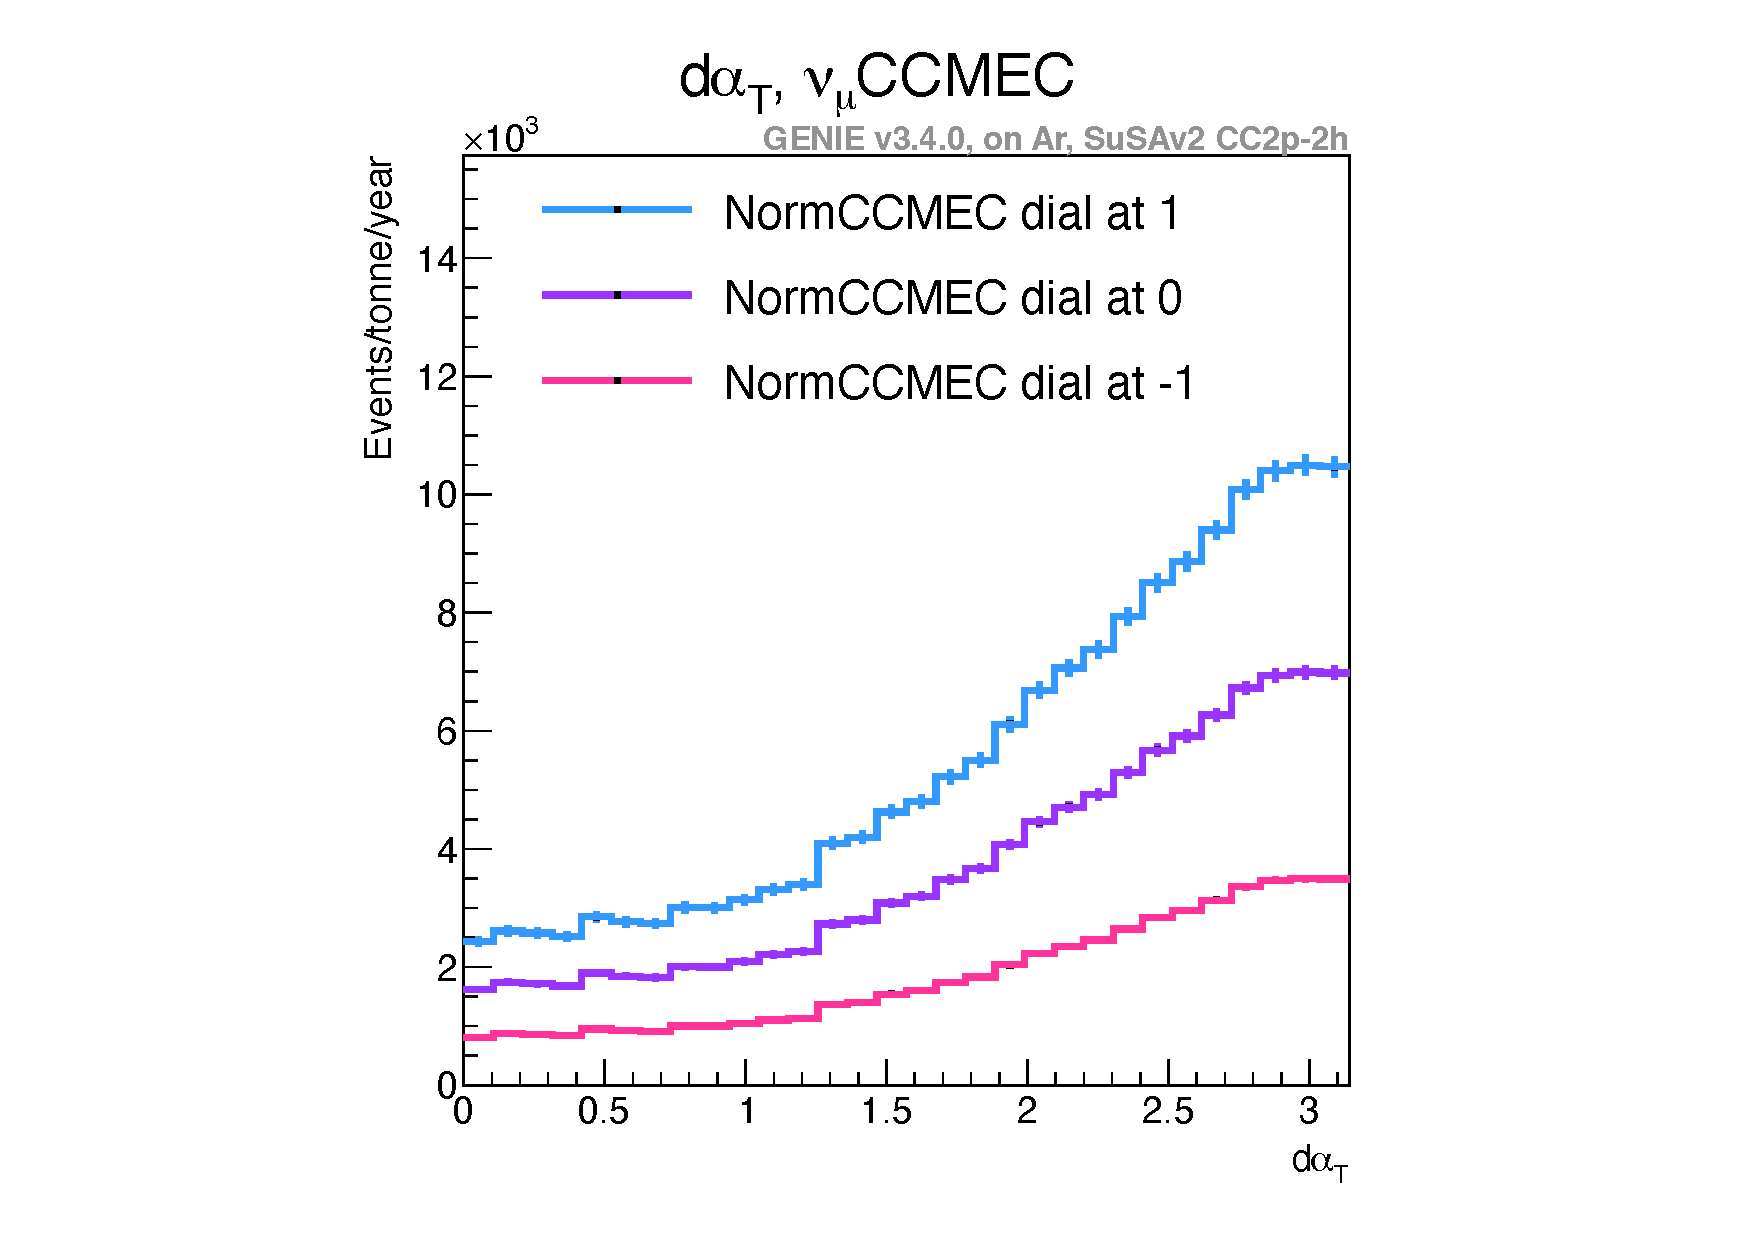
\includegraphics[width=\textwidth]{figures/Norm_CCMEC/1DComp_dat_14_ccmec_edited.pdf}
%        \vspace{-6.mm}
%	\caption{}
	\label{normccmec_b}
    \end{subfigure}
	\begin{subfigure}[b]{.32\textwidth}
%        
\includegraphics[width=\textwidth]{figures/Norm_CCMEC/1DComp_dat_14_ccmec.pdf}
        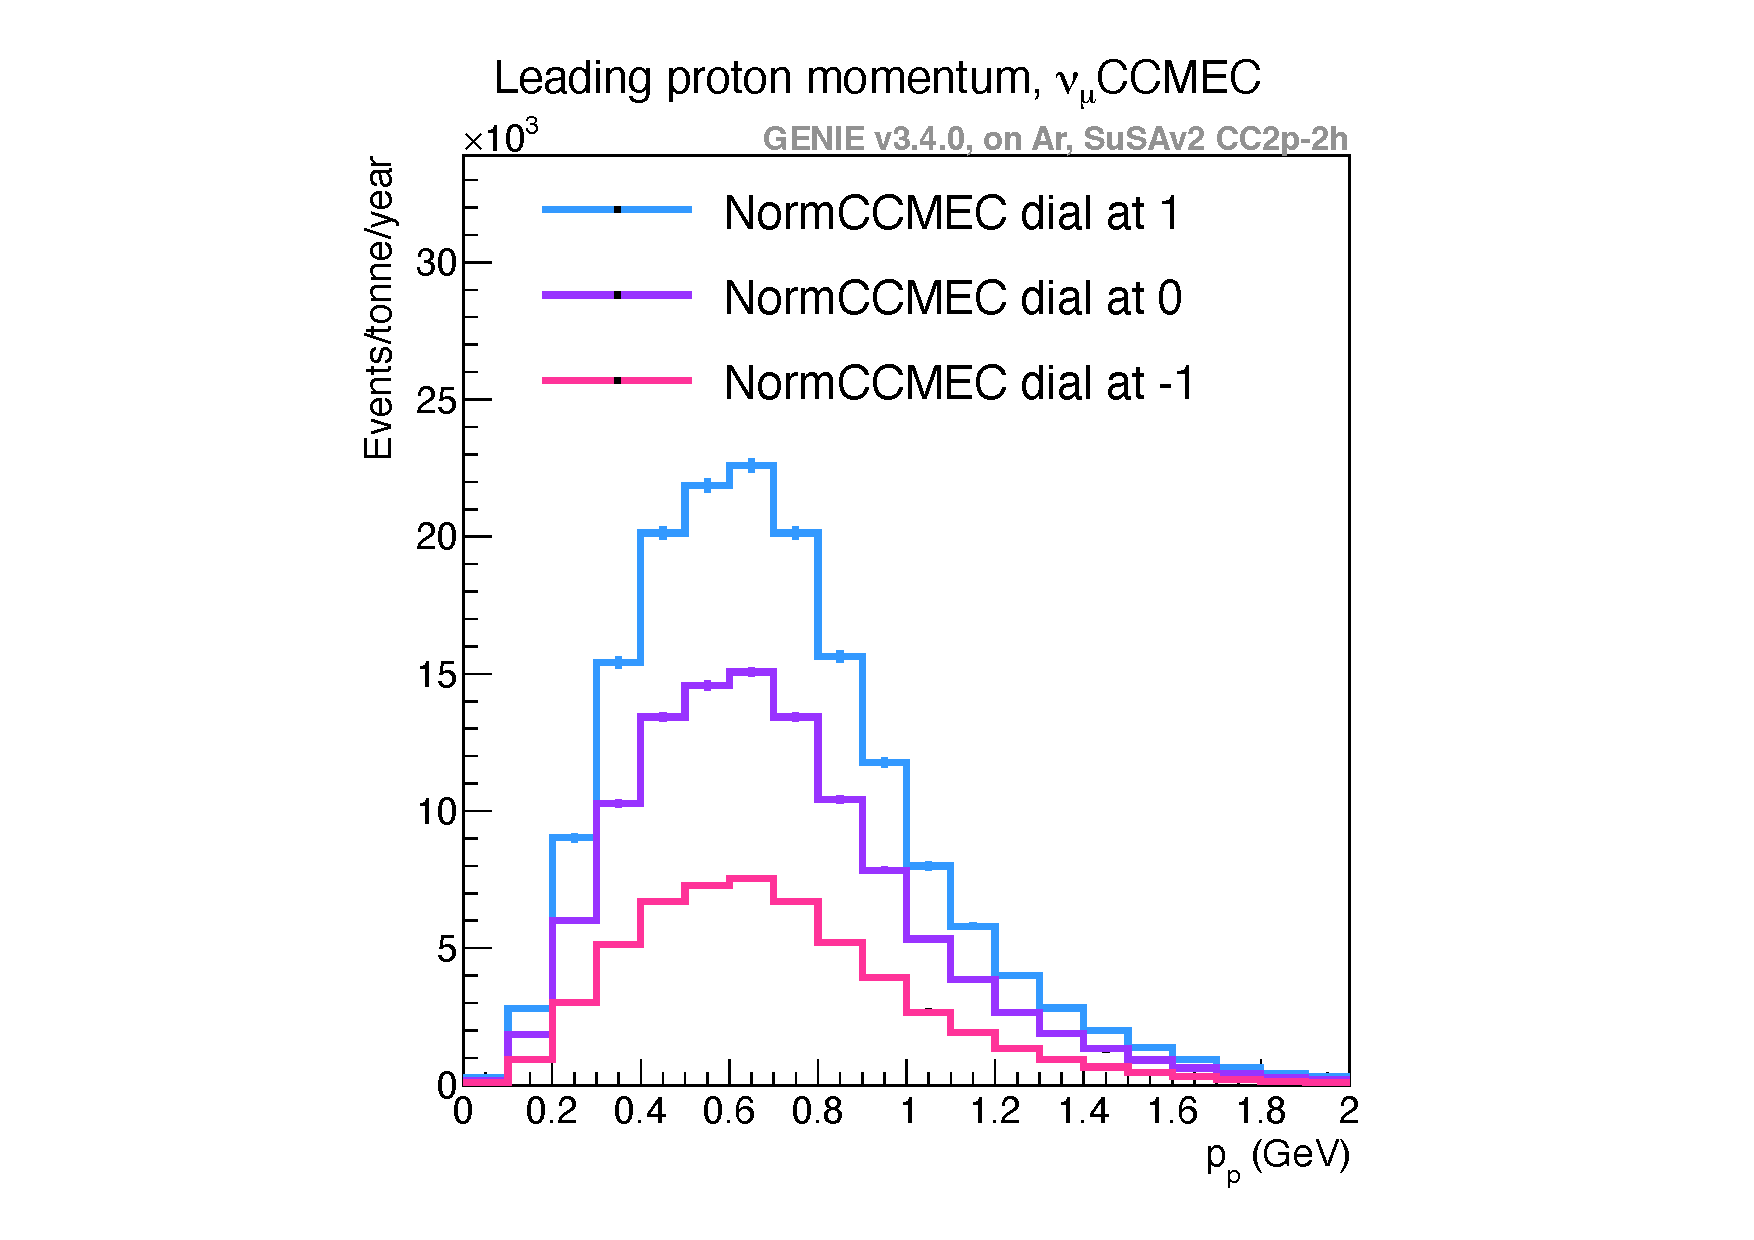
\includegraphics[width=\textwidth]{figures/Norm_CCMEC/1DComp_LeadP_p_14_ccmec_edited.pdf}
%        \vspace{-6.mm}
%	\caption{}
	\label{normccmec_c}
    \end{subfigure}
    \vspace{-6mm}
	\caption[]{NormCCMEC dials for the (left) lepton kinematic $\cos(\theta)_\text{lep}$, (middle) the hadron kinematic variable $p_p$ and (right) the transverse-kinematic angular imbalance $\mathrm{d}\alpha_T$.}
	\label{normccmec}
\end{figure}
\vspace{-1mm}%
As expected, the tweaking of the $\verb!NormCCMEC!$ parameter changes the overall normalisation with respect to the central value configuration and leaves the shape of the distributions unchanged.
\vspace{-3mm}
%
\paragraph{DecayAngMEC}
The \acrshort{cc} \acrshort{2p2h} models described above are inclusive meaning that they only predict the particle kinematics of the outgoing lepton. In the so-called nucleon cluster model \cite{10.1063/1.4919465}, a bound pair of two nucleons is sampled independently from the nuclear ground state distribution and treated as a single object. The leptonic $4$-momentum transfer of the neutrino interaction is imparted on this two-nucleon hadronic final state which then decays to two outgoing nucleons. In the current GENIE \acrshort{cc} \acrshort{2p2h} implementations, the decay angle of these two outgoing nucleons in their rest frame follows an isotropic angular distribution. However, this assumption may be challenged by the $\verb!DecayAngMEC!$ parameter which introduces an angular dependence on the final-state particle kinematics. Hereby, a \acrshort{cc} \acrshort{2p2h} $\verb!DecayAngMEC!$ dial at $0$ resembles the default isotropic distribution, whereas a dial at $1$ yields an angular dependence proportional to $\cos^2(\theta)$ (as a rather anisotropic distribution), where $\theta$ is measured with respect to the $3$-momentum transfer $\mathbf{q}$. Values in between $0$ and $1$ correspond to linear interpolations between these two distributions \cite{PhysRevD.105.072001}.
%\vspace{-2mm}%
\begin{figure}[htb!]
	\begin{subfigure}[b]{.325\textwidth}
%        \includegraphics[width=\textwidth]{figures/DecayAngMEC/1DComp_cosThetaLep_14_ccmec.pdf}
        %
\includegraphics[width=\textwidth]{figures/DecayAngMEC/1DComp_cosThetaLep_14_ccmec_edited.pdf}
        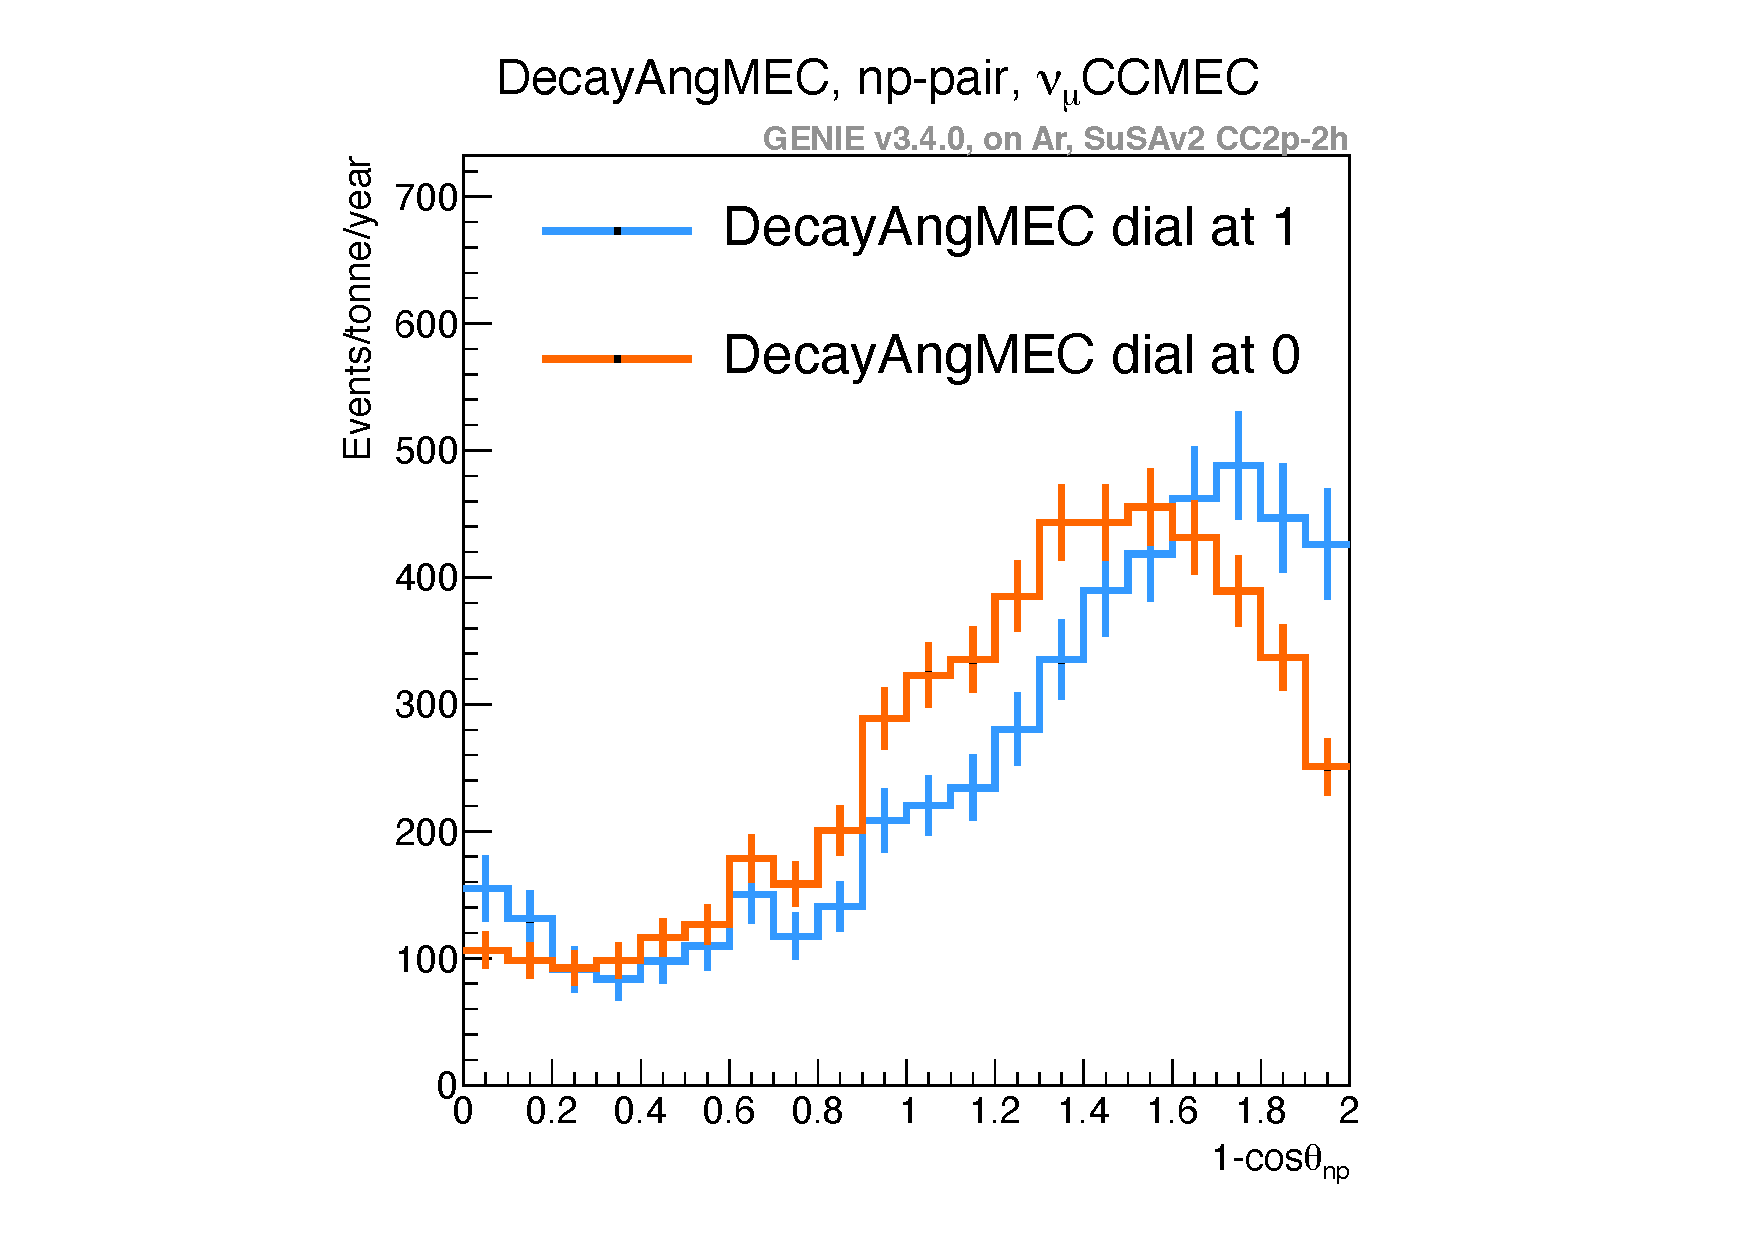
\includegraphics[width=\textwidth]{figures/DecayAngMEC/1DComp_DecayAngMECNP_14_ccmec_edited.pdf}
%        \vspace{-6.mm}
%	\caption{}
	\label{decayangmec_a}
    \end{subfigure}
	\begin{subfigure}[b]{.313\textwidth}
%        \includegraphics[width=\textwidth]{figures/DecayAngMEC/1DComp_LeadP_p_14_ccmec.pdf}
        %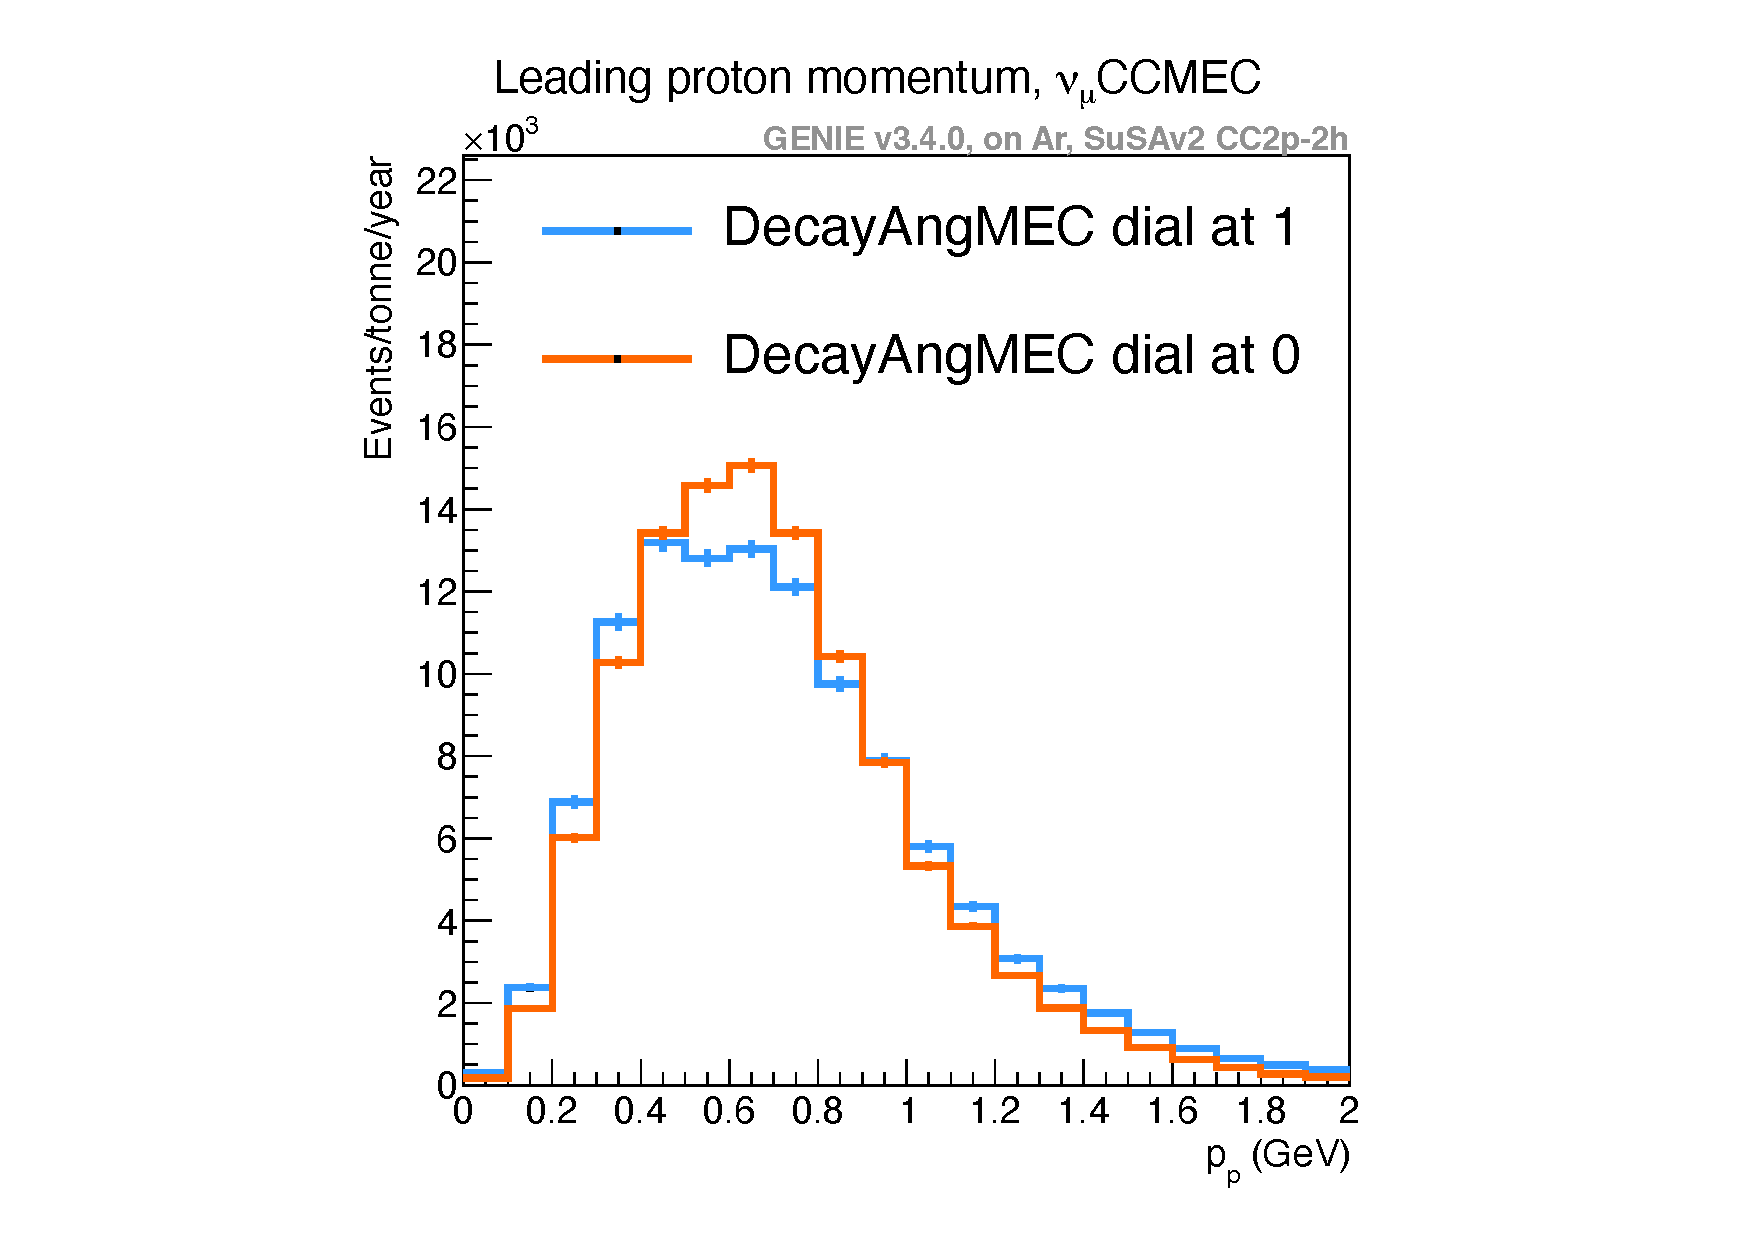
\includegraphics[width=\textwidth]{figures/DecayAngMEC/1DComp_LeadP_p_14_ccmec_edited.pdf}
        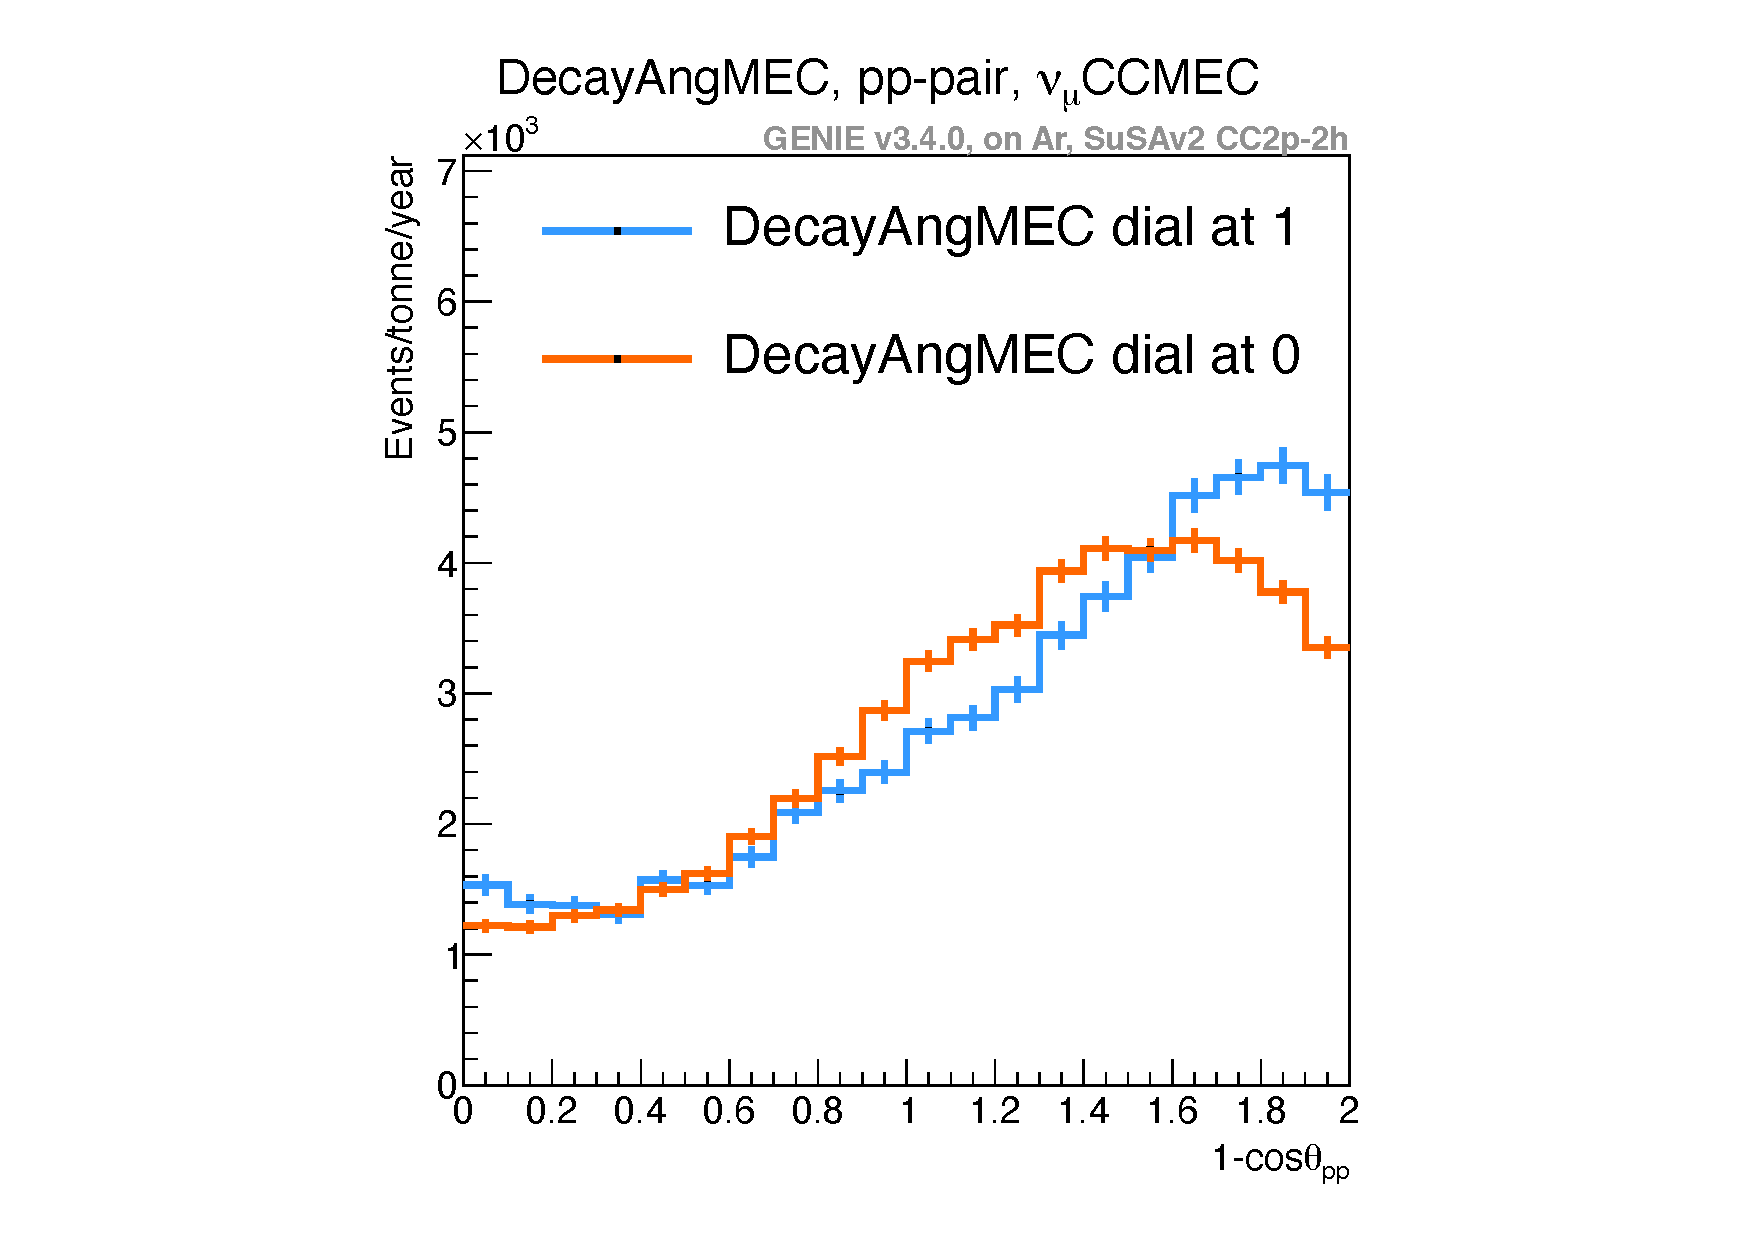
\includegraphics[width=\textwidth]{figures/DecayAngMEC/1DComp_DecayAngMECPP_14_ccmec_edited.pdf}
%        \vspace{-6.mm}
%	\caption{}
	\label{decayangmec_b}
    \end{subfigure}
	\begin{subfigure}[b]{.323\textwidth}
%        
\includegraphics[width=\textwidth]{figures/DecayAngMEC/1DComp_dat_14_ccmec.pdf}
        %
\includegraphics[width=\textwidth]{figures/DecayAngMEC/1DComp_dat_14_ccmec_edited.pdf}
        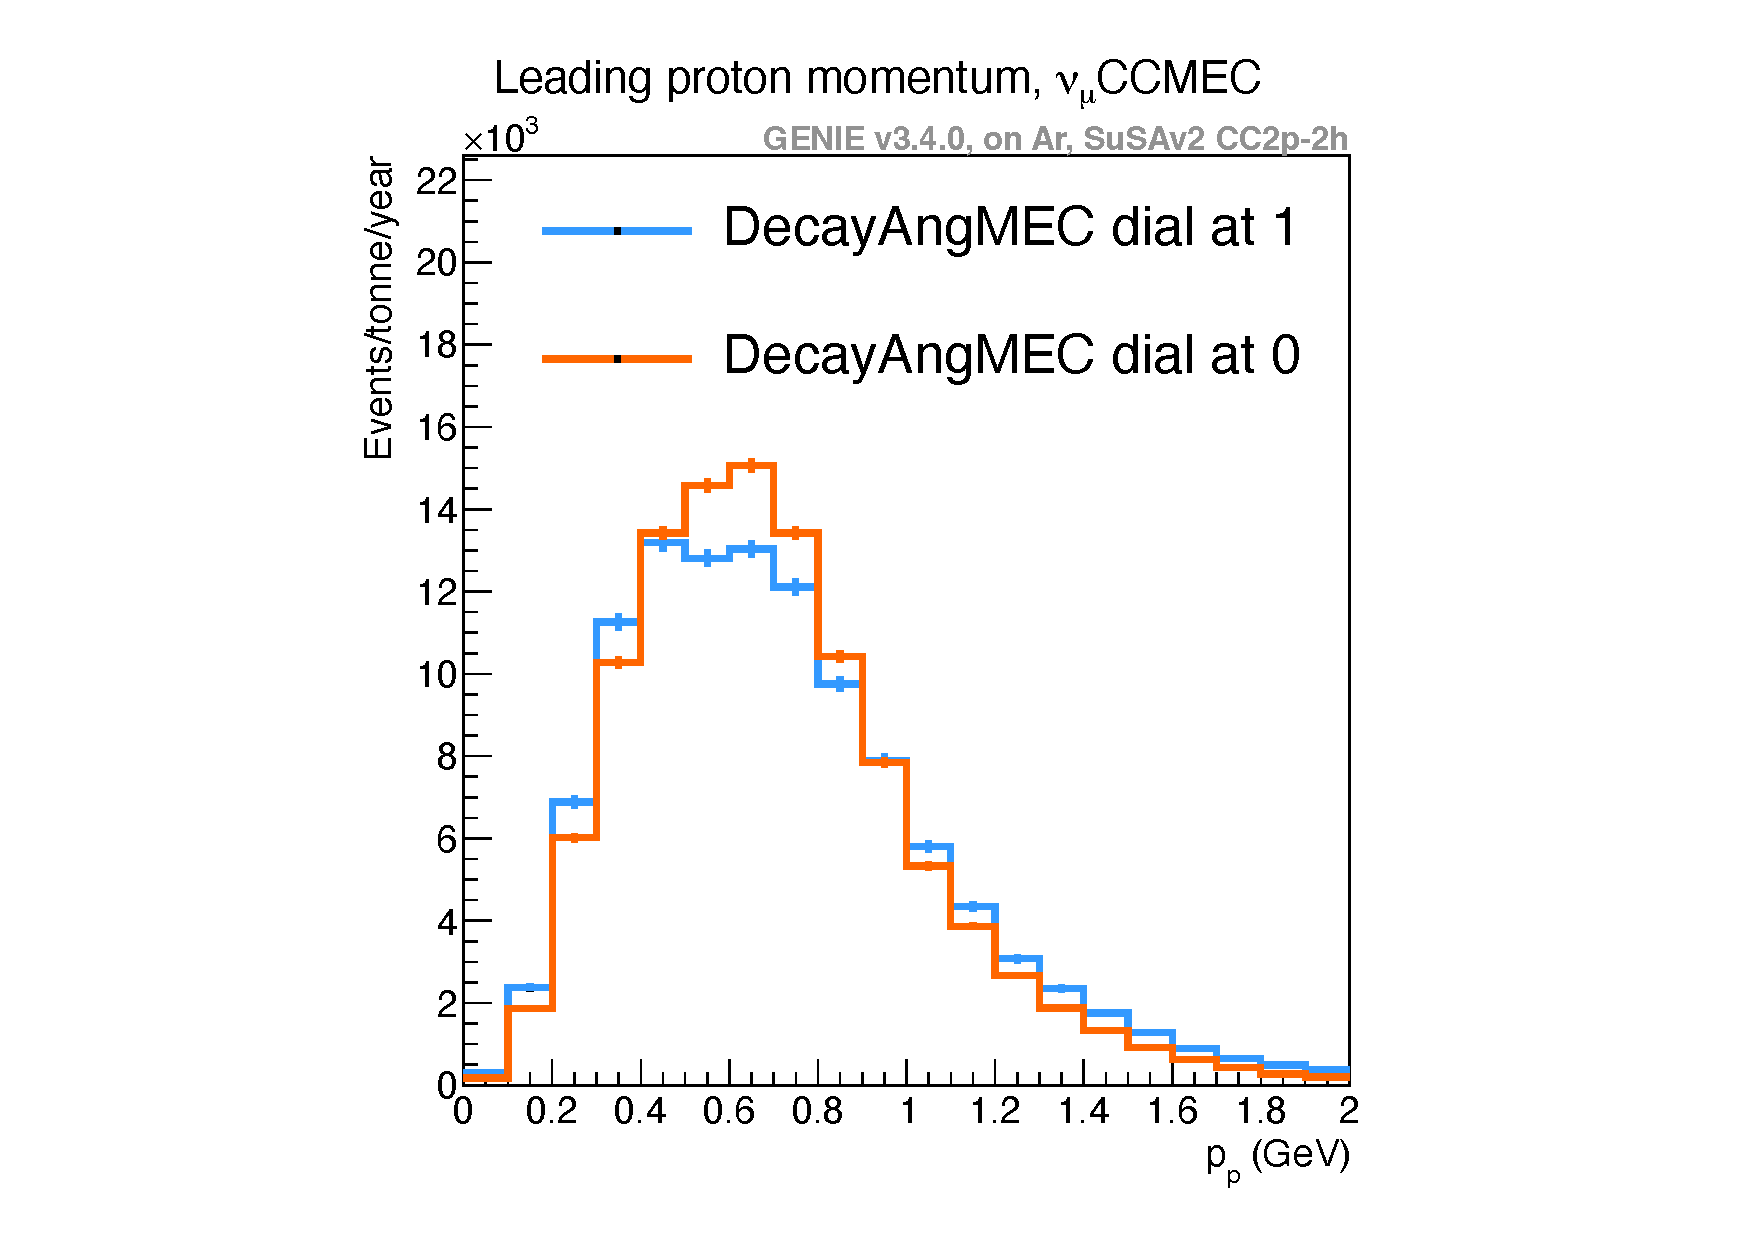
\includegraphics[width=\textwidth]{figures/DecayAngMEC/1DComp_LeadP_p_14_ccmec_edited.pdf}
%        \vspace{-6.mm}
%	\caption{}
	\label{decayangmec_c}
    \end{subfigure}
    \vspace{-6mm}
	\caption[]{DecayAngMEC dials for $1-\cos(\theta_\text{lep})$ for different bound final states and (right) $p_p$.}
	\label{decayangmec}
\end{figure}
%\vspace{-1mm}%
The tuning of the $\verb!DecayAngMEC!$ %as well as the $\verb!FracPN_CCMEC!$ 
systematic parameter have relatively small effects on the distributions shown in \cref{decayangmec}. However, there are subtle differences in the distributions for the decay angle between the struck nucleons in dependence on whether the final-state of the interaction was a np- or pp-pair (see \cref{decayangmec} (left) and (middle)). The change of the leading proton momentum distribution in \cref{decayangmec} (right) is modest, as it would be expected, since this dial represents a physical effect regarding the outgoing nucleons only.  %Though a combined measurement of this leptonic kinematic variable distribution with the leading proton momentum distriblution may allow one to find a region of phase space that provides discrimination potential between the three models. 
\vspace{-3mm}
\paragraph{FracPN\_CCMEC}
A \acrshort{cc} \acrshort{2p2h} interaction occurs on an initial pair of nucleons that either share the same third component of isospin (a nn-bound state of two neutrons for neutrinos and a pp-pair for antineutrinos) or different isospin (a pn-bound state of one neutron and one proton). The $\verb!FracPN_CCMEC!$ parameter adopts a fractional uncertainty of $\pm20\%$ by adjusting the fraction of events involving an initial pn pair relative to the default prediction of the input \acrshort{cc} \acrshort{2p2h} model \cite{PhysRevD.105.072001}.
%\vspace{-2mm}%
\begin{figure}[htb!]
	\begin{subfigure}[b]{.319\textwidth}
%        \includegraphics[width=\textwidth]{figures/FracPN_CCMEC/1DComp_cosThetaLep_14_ccmec.pdf}
        %
\includegraphics[width=\textwidth]{figures/FracPN_CCMEC/1DComp_cosThetaLep_14_ccmec_edited.pdf}
        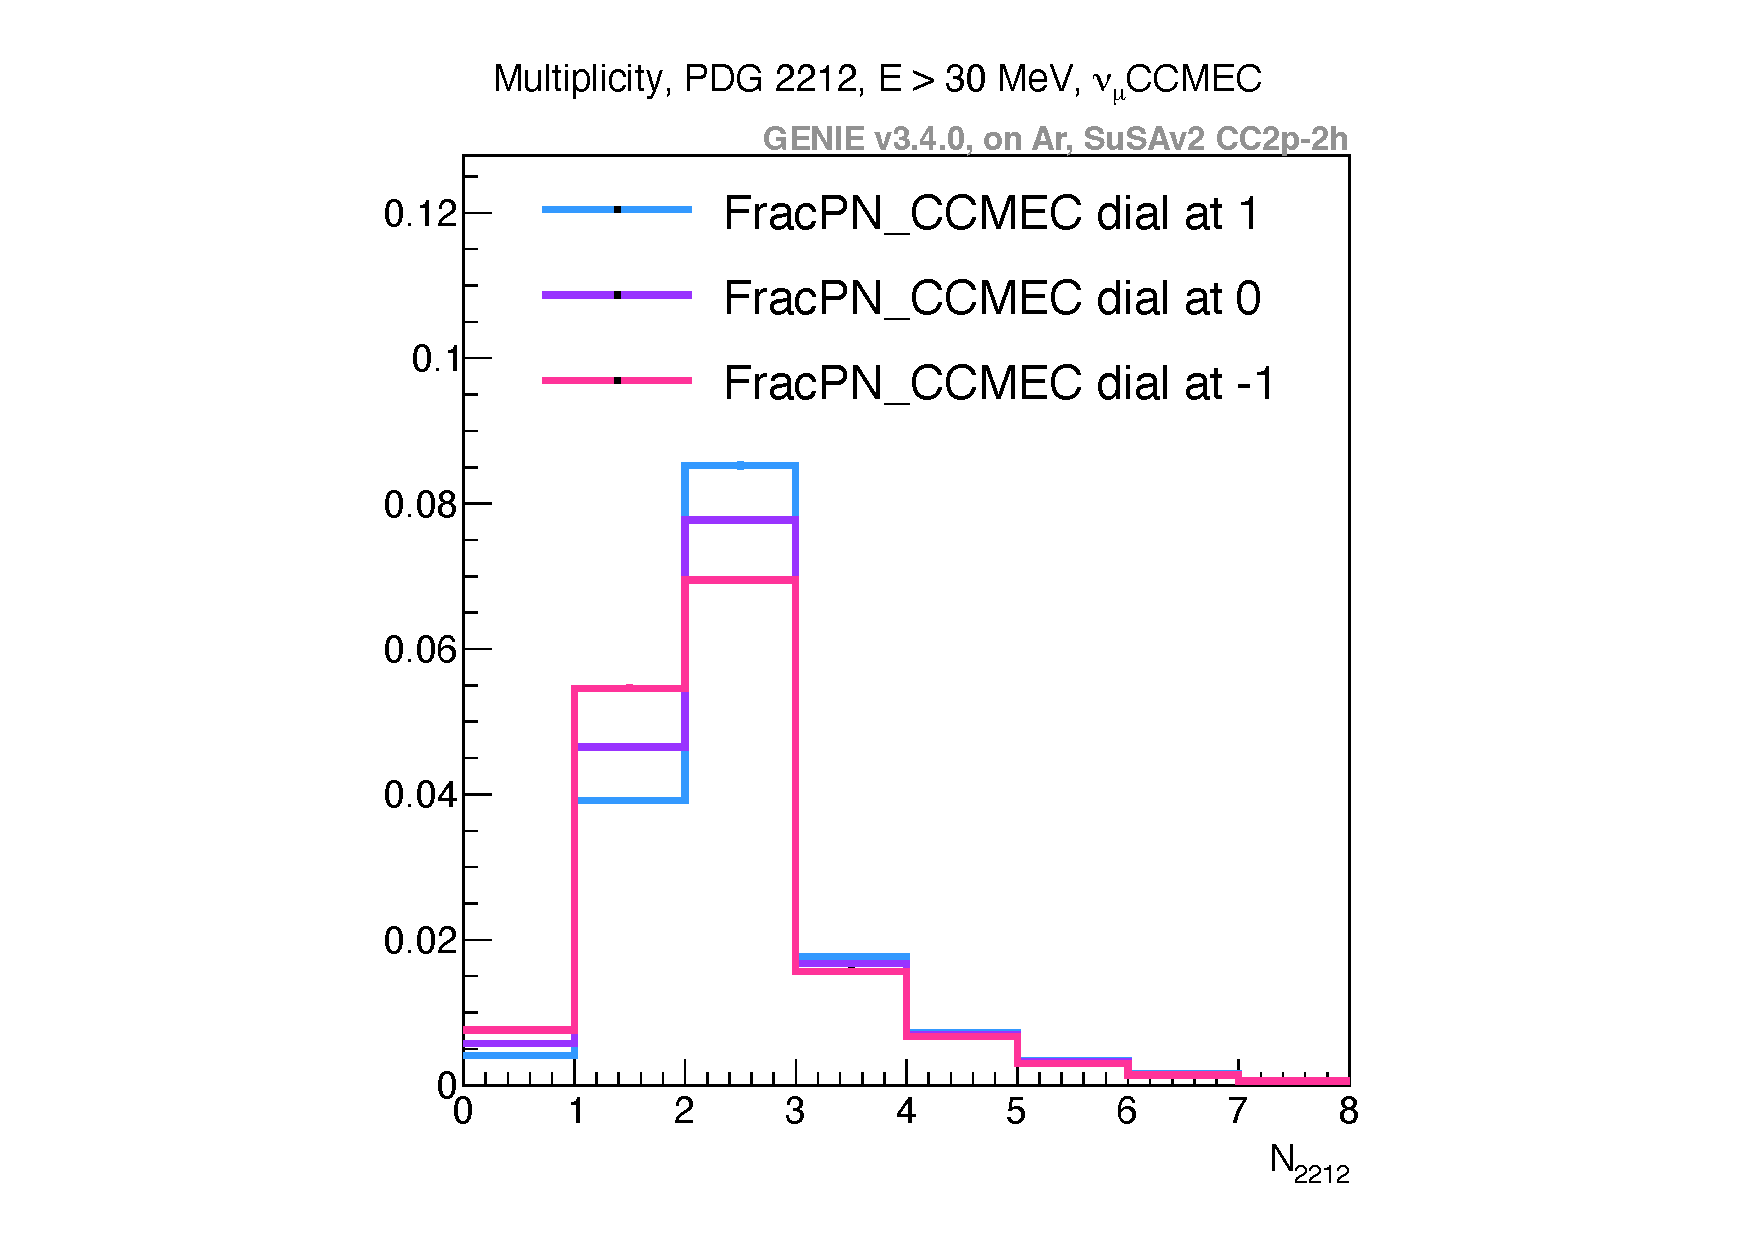
\includegraphics[width=\textwidth]{figures/FracPN_CCMEC/1DComp_mult_2212_14_ccmec_multp_30MeV_edited.pdf}
        %\includegraphics[width=\textwidth]{figures/FracPN_CCMEC/1DComp_mult_2212_14_ccmec_multp_30MeV_edited2.pdf}
        %\includegraphics[width=\textwidth]{figures/FracPN_CCMEC/1DComp_mult_2212_14_ccmec_multp_30MeV_edited3.pdf}
%        \vspace{-6.mm}
%	\caption{}
	\label{fracpnccmec_a}
    \end{subfigure}
	\begin{subfigure}[b]{.332\textwidth}
%        \includegraphics[width=\textwidth]{figures/FracPN_CCMEC/1DComp_LeadP_p_14_ccmec.pdf}
        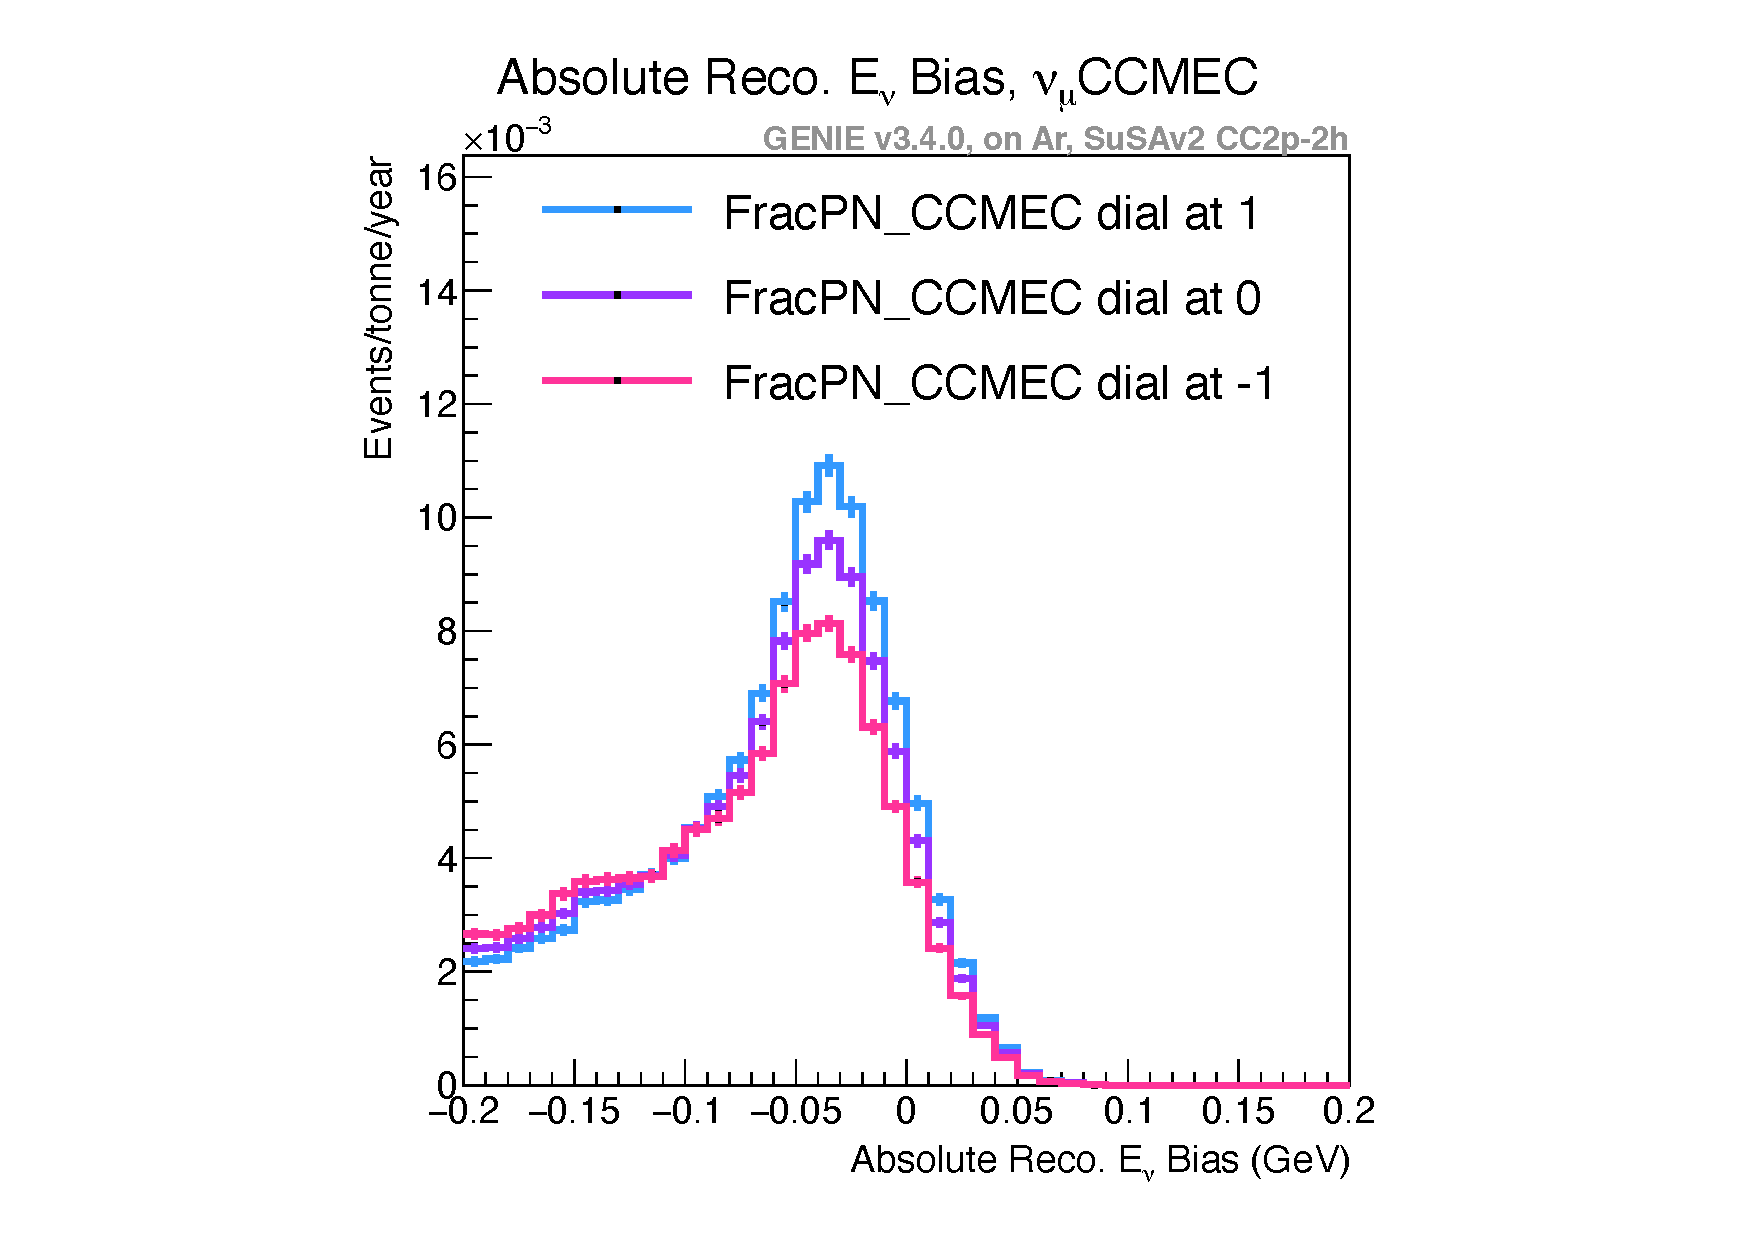
\includegraphics[width=\textwidth]{figures/FracPN_CCMEC/1DComp_ErecAbsBias_14_ccmec_edited.pdf}
%        \vspace{-6.mm}
%	\caption{}
	\label{fracpnccmec_b}
    \end{subfigure}
	\begin{subfigure}[b]{.328\textwidth}
%        
\includegraphics[width=\textwidth]{figures/FracPN_CCMEC/1DComp_dat_14_ccmec.pdf}
        %
\includegraphics[width=\textwidth]{figures/FracPN_CCMEC/1DComp_dat_14_ccmec_edited.pdf}
        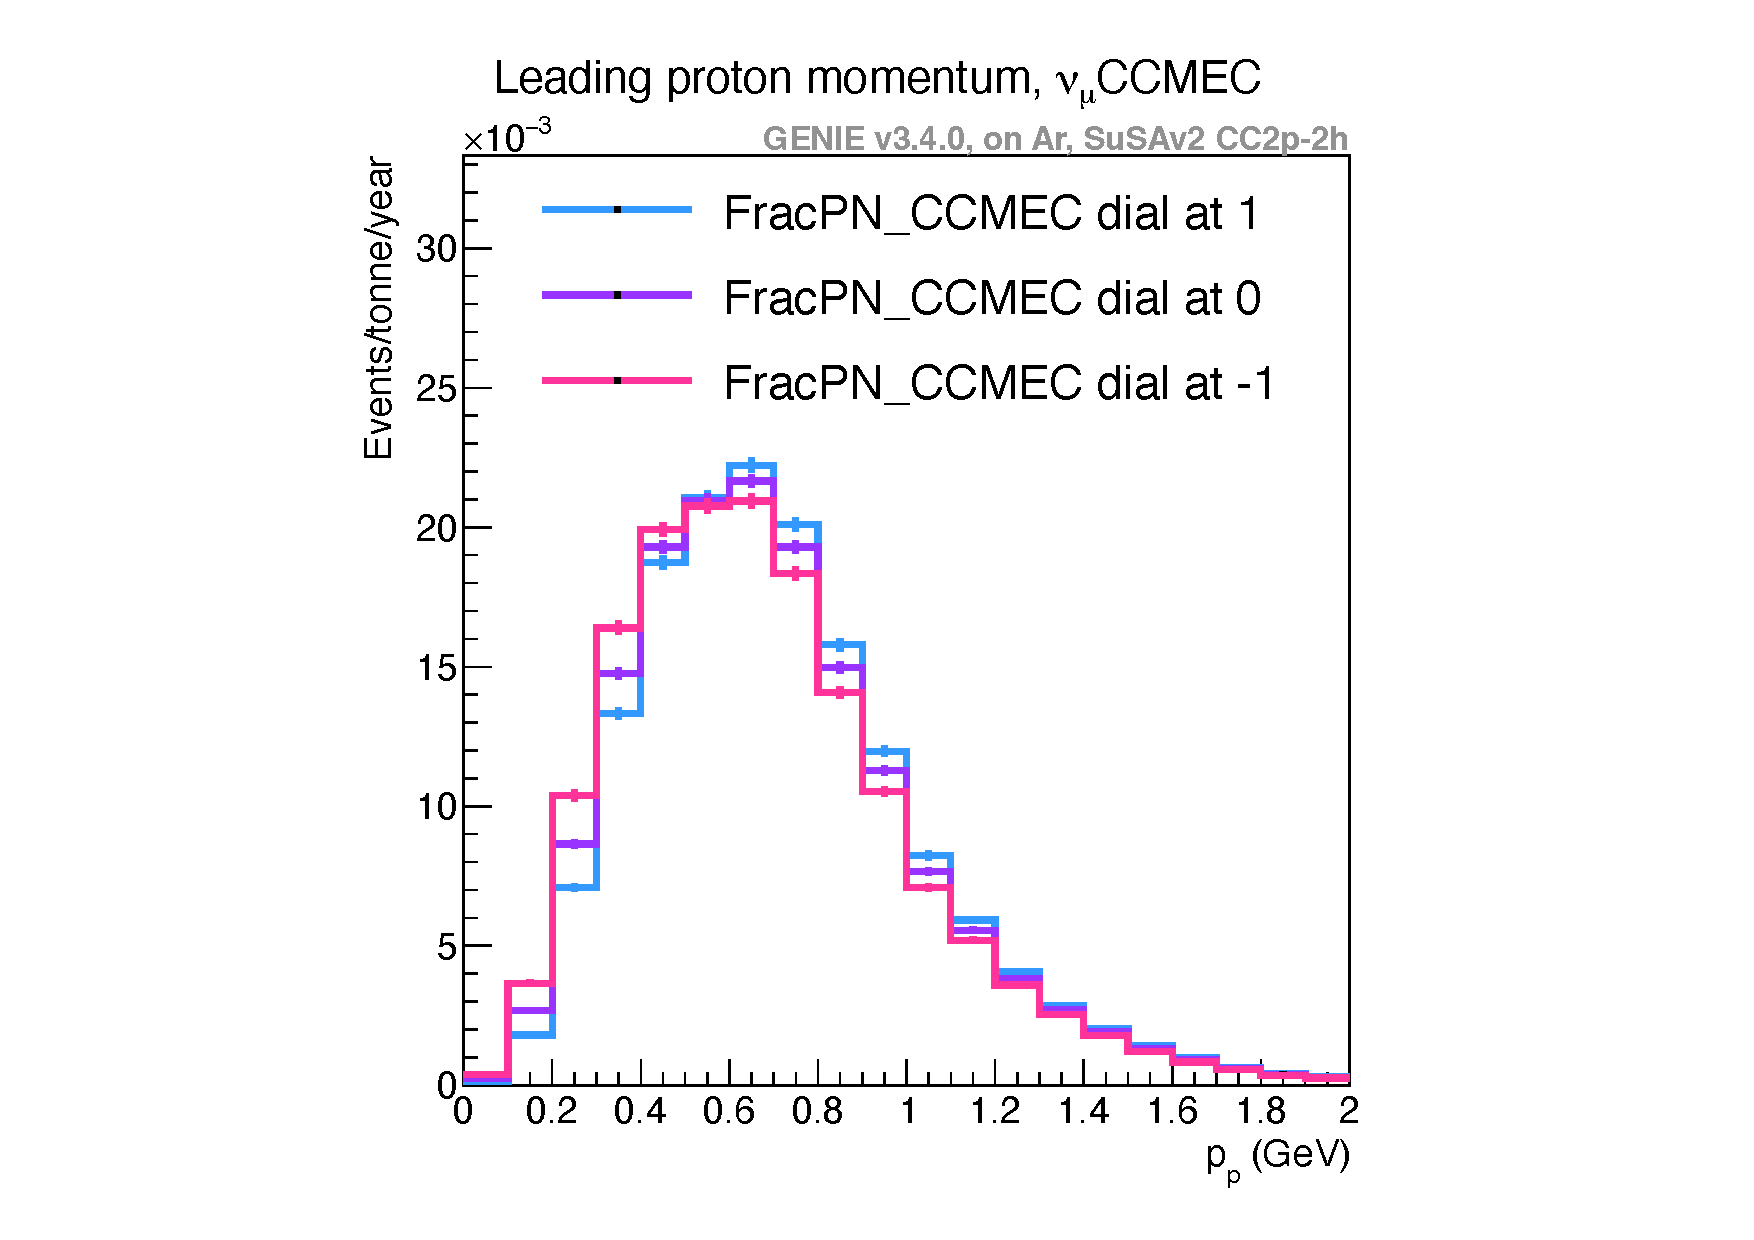
\includegraphics[width=\textwidth]{figures/FracPN_CCMEC/1DComp_LeadP_p_14_ccmec_edited.pdf}
%        \vspace{-6.mm}
%	\caption{}
	\label{fracpnccmec_c}
    \end{subfigure}
    \vspace{-6mm}
	\caption[]{FracPN\_CCMEC dials for proton multiplicity, energy bias and $p_p$ (from left to right).}
	\label{fracpnccmec_plots}
\end{figure}
%\vspace{-1mm}%
The changing of the $\verb!FracPN_CCMEC!$ parameter either raises (positive dial) or lowers (negative dial) the pn-pair content (and hence lowers the nn-pair content) in the initial nuclear state. Hence moving away from the $\verb!FracPN_CCMEC!$ central value at $0$ leads to more protons with measurable energies for \acrshort{dune} above $E_\nu>30$MeV being observed in \cref{fracpnccmec_plots} (left) and hence also more visible energy in \cref{fracpnccmec_plots} (middle) (as a neutrons cannot be detected). It is also possible to see related effects in \cref{fracpnccmec_plots} (right).
\vspace{-3mm}
\paragraph{XSecShape\_CCMEC} \label{xsecshapeccmec_paragraph}
Currently there are substantial differences between alternative theoretical predictions of lepton kinematics on \acrshort{cc} \acrshort{2p2h} scattering in dependence on the chosen model. In order to investigate the currently unknown \acrshort{cc} \acrshort{2p2h} cross-section shape, the $\verb!XSecShape_CCMEC!$ parameter changes the shape of the inclusive \acrshort{cc} \acrshort{2p2h} differential cross section between the GENIE Empirical model \cite{10.1063/1.4919465}, the Valencia model \cite{PhysRevD.88.113007} and the SuSAv$2$ model \cite{Amaro_2020}. By setting the $\verb!XSecShape_CCMEC!$ parameter, a linear interpolation allows for continuous variabtions fo the dial in order to explore the shape of respective distributions and how they change shape when renormlising the distributions from one model shape to another. These shape dial variations and their effects on chosen variable distributions can be seen in \cref{xsecshapeccmec}.
The $\verb!XSecShape_CCMEC!$ parameter allows one to observe continuosly varied simulation predictions in between the three \acrshort{cc} \acrshort{2p2h} models. %Hence, when performing a measurement within \acrshort{dune}, these simulations may give hints on whether one model provides a more successful description of nature in some phase space region as opposed to another model perhaps being more reliable in another region of phase space. 
%\vspace{-5mm}%
\begin{figure}[htb!]
	\begin{subfigure}[b]{.32\textwidth}
%        \includegraphics[width=\textwidth]{figures/XSecShape_CCMEC/1DComp_cosThetaLep_14_ccmec.pdf}
        %
\includegraphics[width=\textwidth]{figures/XSecShape_CCMEC/1DComp_cosThetaLep_14_ccmec_edited.pdf}
        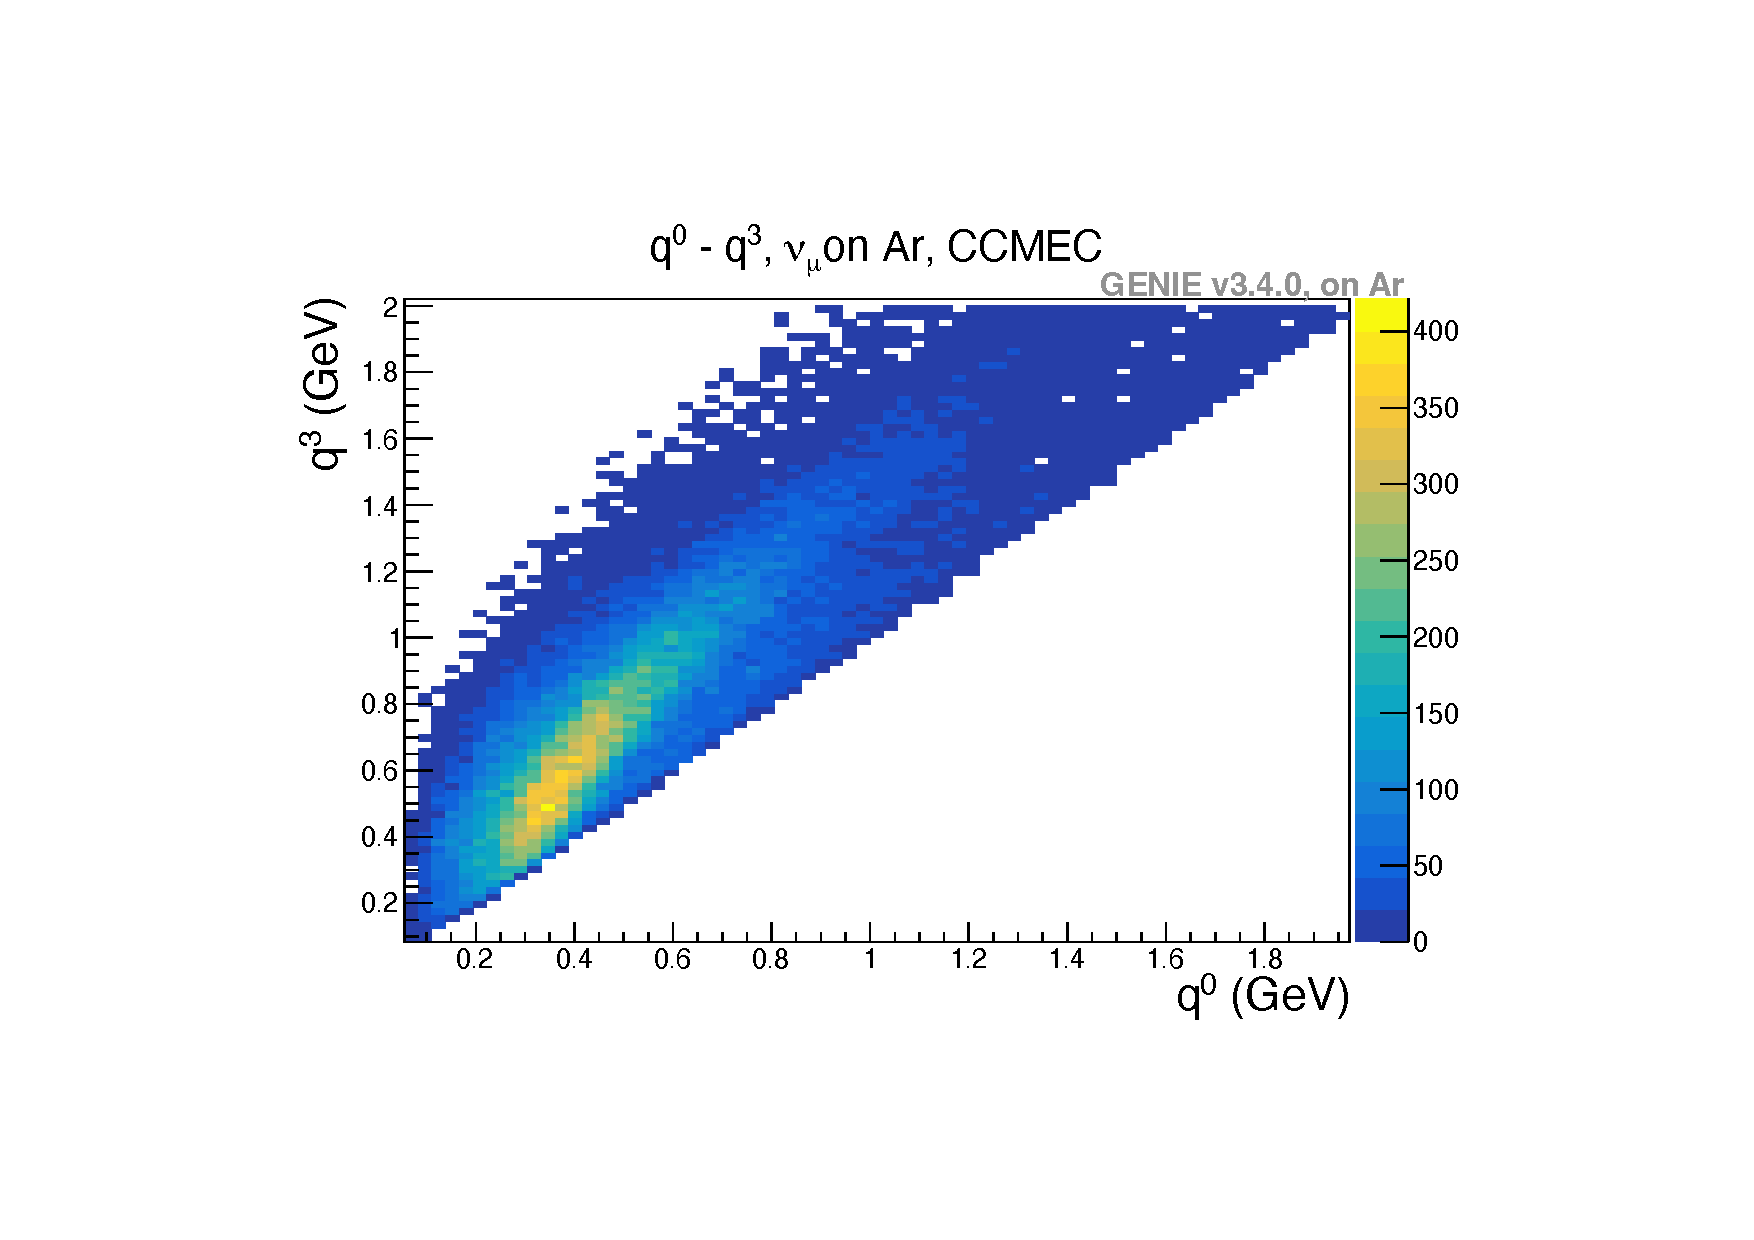
\includegraphics[width=\textwidth]{figures/XSecShape_CCMEC/2DComp_q0-q3_SuSAv2_edited.pdf}
        \vspace{-2.mm}
%	\caption{}
	\label{xsecshapeccmec_a}
    \end{subfigure}
	\begin{subfigure}[b]{.32\textwidth}
%        \includegraphics[width=\textwidth]{figures/XSecShape_CCMEC/1DComp_LeadP_p_14_ccmec.pdf}
        %
\includegraphics[width=\textwidth]{figures/XSecShape_CCMEC/1DComp_LeadP_p_14_ccmec_edited.pdf}
        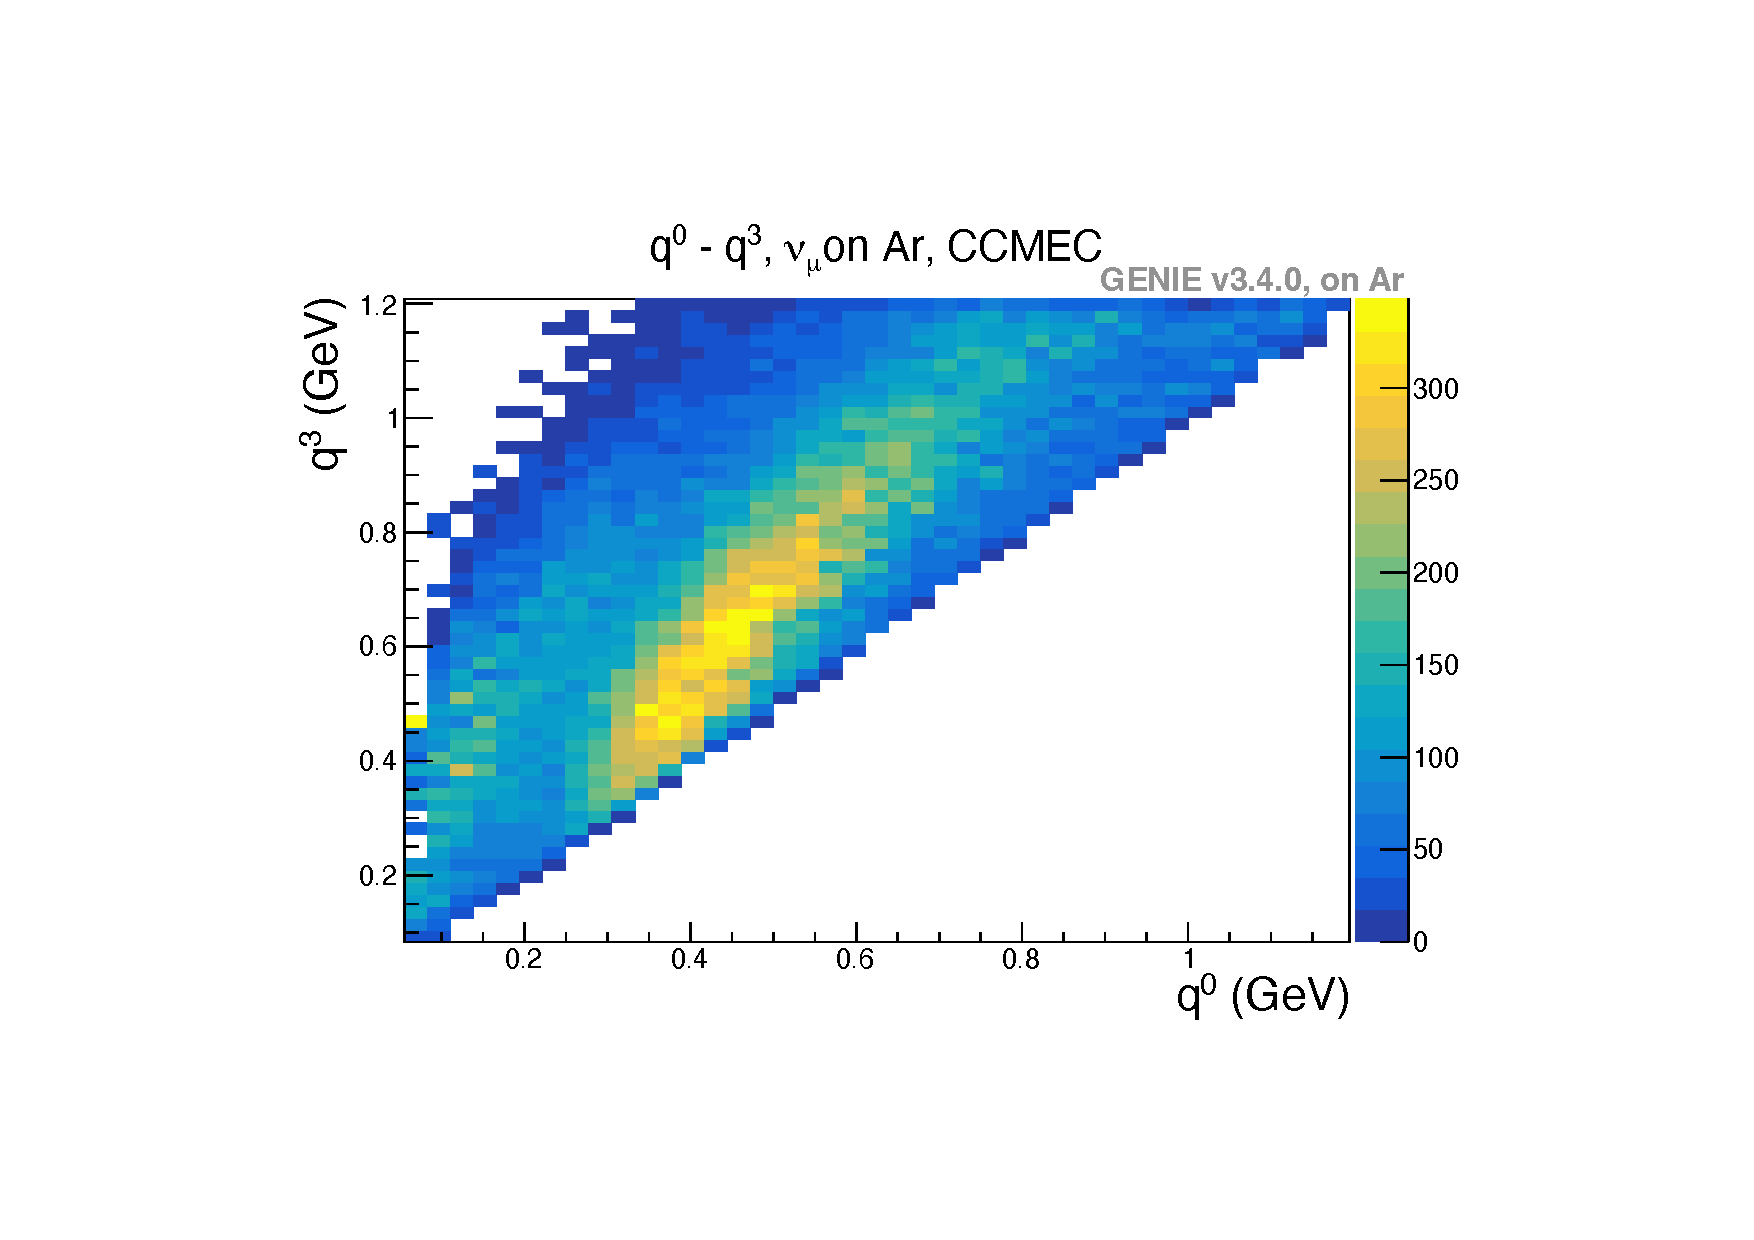
\includegraphics[width=\textwidth]{figures/XSecShape_CCMEC/2DComp_q0-q3_SuSAv2->Valencia_edited.pdf}
        \vspace{-2.mm}
%	\caption{}
	\label{xsecshapeccmec_b}
    \end{subfigure}
	\begin{subfigure}[b]{.32\textwidth}
%        
\includegraphics[width=\textwidth]{figures/XSecShape_CCMEC/1DComp_dat_14_ccmec.pdf}
        %
\includegraphics[width=\textwidth]{figures/XSecShape_CCMEC/1DComp_dat_14_ccmec_edited.pdf}
        %
\includegraphics[width=\textwidth]{figures/XSecShape_CCMEC/1DComp_LeadP_p_14_ccmec_edited.pdf}
        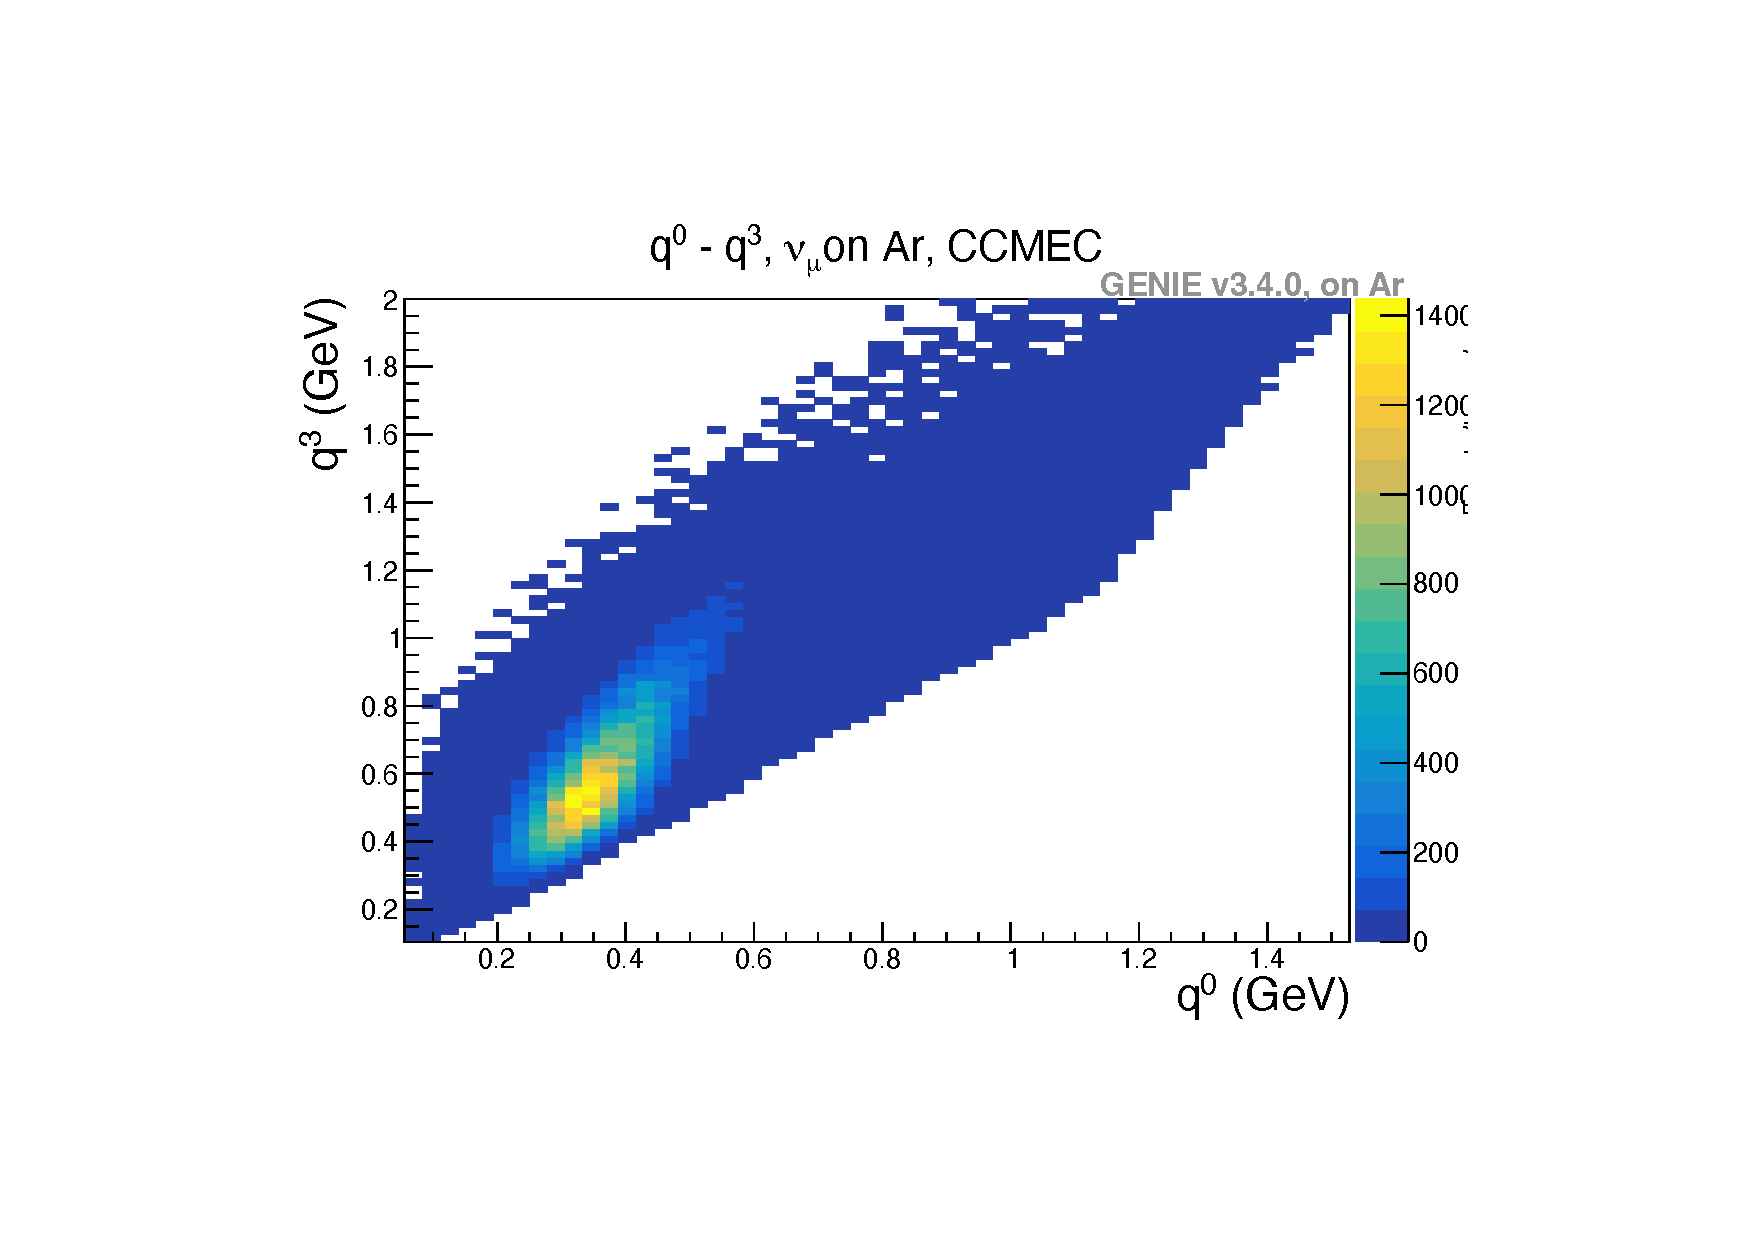
\includegraphics[width=\textwidth]{figures/XSecShape_CCMEC/2DComp_q0-q3_SuSAv2->Empirical_edited.pdf}
        \vspace{-2.mm}
%	\caption{}
	\label{xsecshapeccmec_c}
    \end{subfigure}
    \vspace{-6mm}
	\caption[]{XSecShape\_CCMEC parameter dials. The $q^0-q^3$ distributions are area-normalised.}
	\label{xsecshapeccmec}
\end{figure}
%\vspace{-5mm}%
%Most discrimination potential in the plots shown lie in the leading proton momentum distribution in \cref{xsecshapeccmec_b}. As the distribution is reshaped to resemble the GENIE Empirical model prediction (see \cref{xsecshapeccmec_b}), the peak seen for the SuSAv$2$ calculation gets enhanced and the tail contains less relative events. In dependence on the variable, the change in the shape of these \acrshort{cc} \acrshort{2p2h} distributions is subtle in some regions of phase space, whereas it is prominent in other regions of phase space. \cite{PhysRevD.105.072001}.
Fig. \ref{xsecshapeccmec} shows the $3$-momentum transfer $q^3$ versus the energy transfer $q^0$ for the (left) default SuSAv$2$ ($\verb!XSecShape_CCMEC!$ dial at $0$), the $\verb!XSecShape_CCMEC!$ tweaked dial to the (middle) Valencia as well as the $\verb!XSecShape_CCMEC!$ tweaked dial to the (right) Empirical model prediction. As the SuSAv$2$ model with one visible peak is reshaped to resemble the GENIE Empirical model prediction, the peak seen for the SuSAv$2$ calculation becomes narrower. A reshaping from the SuSAv$2$ to the Valencia model results in the emergence of a second local maximum for low $q^0$ values, which is expected \cite{PhysRevD.105.072001}. %gets enhanced and the tail contains less relative events.

%\subsection{Uncertainty Implementation}

%\newpage
% Analysis of results and conclusions, discussion of plans for future work
\vspace{-4mm}
\section{Conclusion and Outlook} \label{conclusion_syst} \vspace{-3mm}
This report reviewed the importance of understanding nuclear effects and neutrino-nucleus interactions in light of future neutrino oscillation studies. One strategy to address the theoretically-challenging description of the neutrino-nucleus scattering processes lies in the development of systematic fit parameters that can be used to develop enhanced theory-driven simulation predictions. In this study, I analysed the effects of \acrshort{fsi}s on kinematic variable distributions and also differences in three \acrshort{cc} \acrshort{2p2h} models that are currently available in the neutrino event generator GENIE. I have also finished the implementation of four systematic parameter dials that are of great interest for the experimental neutrino physics, especially the \acrshort{dune} collaboration community. %Furthermore, these dials have been discussed beyond the scope of \acrshort{dune}, for example in the T$2$K collaboration. 
The effects of these dials on chosen variable distributions was examined and validated. This will allow a robust estimate of systematic uncertainties in the \acrshort{dune} oscillation analysis. It will also allow one to take into account differences between models as well as uncertainties within a single model. Moreover, since other experimental neutrino physics collaborations such as T$2$K are as well interested in reweighting fitting parameters for propagating uncertainties, this analysis is expected to be of great importance beyond the scope of \acrshort{dune}. After making these dials publicly available as part of GENIEReweight, the goal is to obtain improved systematic uncertainties for better sensitivities in the \acrshort{dune} neutrino oscillation analysis, which will be the next task as part of my DPhil project.
%dials finalised-> pull request to GENIE, present work to GENIE collaboration, accept it as part of GENIE; present to DUNE, new systemstics for DUNE oscialltion sensititvities; work on oscillations and sensitivities in DUNE